\documentclass{templateRevistaUPTCCiencias}
%\usepackage{templateRevistaUPT}
\usepackage{times,mathptmx}
\usepackage{lastpage}
\usepackage{booktabs}
\usepackage{fancyhdr}
\usepackage{minted}
\usepackage{titlesec}
\titleformat{\section}
  {\normalfont\large\bfseries\centering}
  {\thesection}
  {1em}
  {}
\pagestyle{fancy}
% -------------------------------------------------------------------------------------
% Plantilla de un art\'iculo para publicar en la Revista Ciencia en Desarrollo
% *************************************************************************************
%
% -------------------------------------------------------------------------------------
% Espacio reservado para la carga de los paquetes por parte del autor
% **** --------------------------------------------------------------------------------
\usepackage[T1]{fontenc}
\usepackage{selinput}
\SelectInputMappings{
	aacute={á}
}

% Las siguientes dos lineas las usamos para generar las referencias
% automaticamente
\usepackage[round]{natbib}
\bibliographystyle{abbrvnat}

\usepackage{bm} % Para usar bold en letras griegas con \bm{}
\usepackage{minted} % Code Highlighting with minted

\usepackage[english]{babel}
%\decimalpoint   % Para que los decimales fueran puntos

\usepackage{hyperref} % Para usar hyper enlaces

\usepackage{minted} % Code Highlighting with minted

\usepackage{multirow} % Para celdas que ocupan varias filas en las tablas


% //// --------------------------------------------------------------------------------
% -------------------------------------------------------------------------------------
% Espacio reservado para colocar las definiciones especiales por parte del autor
% **** --------------------------------------------------------------------------------
% Nombres en español para figuras, tablas y referencias (el artículo está en español)
% Enlaces y citas sin recuadros de colores
\hypersetup{hidelinks}

\addto\captionsenglish{%
  \renewcommand{\figurename}{Figura}%
  \renewcommand{\tablename}{Tabla}%
  \renewcommand{\refname}{Referencias}%
}

% //// --------------------------------------------------------------------------------
% -------------------------------------------------------------------------------------
% Espacio utilizado para colocar las palabras que necesitan partici\'on sil\'abica
% **** --------------------------------------------------------------------------------
\hyphenation{Colombia mul-ti-va-ria-do pro-ba-bi-li-dad es-ta-d\'is-ti-ca}
% //// --------------------------------------------------------------------------------

\begin{document}
\fancypagestyle{plain}% Para la primera p\´agina
{%
\fancyhf{}
\renewcommand{\headrulewidth}{0.5pt}
\renewcommand{\footrulewidth}{0pt}
\fancyheadoffset[RE,LO]{-0.57\textwidth}
\fancyhead[RO]{
\includegraphics[scale=0.045]{logo cienciaendesarrollo-01.jpg}} %\footnotesize{Revista Ciencia en Desarrollo}}
\fancyhead[LO]{Vol. 12 (n\'um. 1)\\ Enero-Junio 2021}
\fancyfoot[CO]{\footnotesize{\thepage}}
}


\fancyhead{}
%\fancyhead[CE]{\footnotesize{Hernández-Barajas, et al.}}
\fancyhead[CO]{\footnotesize{EFICIENCIA HIDRÁULICA DE RODETES PELTON Y TURGO}}

\fancyfoot{}
\fancyfoot[RO]{\footnotesize{\thepage}}
\fancyfoot[LE]{\footnotesize{\thepage}}
\renewcommand{\headrulewidth}{1pt}
\setlength{\columnsep}{6.5mm}

%-------------------------------------------------------------------------------------
% Espacio reservado para ingresar el t\'itulo del art\'iculo
%--------------------------------------------------------------------------------
\title{Modelos de regresión para la eficiencia hidráulica de rodetes Pelton y Turgo de eje vertical}
\subtitle{Regression models for the hydraulic efficiency of vertical-axis Pelton and Turgo runners}
\author{
María Paula Ardila Otero$^{1,*}$\\
\small{$^{1}$Estudiante de Ciencias de la Computación y de Estadística, Universidad Nacional de Colombia sede Medellín, Medellín, Colombia, mardilao@unal.edu.co}\\
\small{\texttt{$^{*}$mardilao@unal.edu.co}}
}
\onecolumn
\maketitle

\footnotetext[1]{$^{*}$Author to whom correspondence 
should be addressed.}

% //// --------------------------------------------------------------------------------
% -------------------------------------------------------------------------------------
% CUERPO DEL DOCUMENTO
% **** --------------------------------------------------------------------------------
% -------------------------------------------------------------------------------------
% Espacio reservado para colocar el resumen en el idioma principal y las palabras clave
% No dejar salto de l\'inea entre el resumen y el comando \keywords{.}¡
% **** --------------------------------------------------------------------------------
% ------------------------------------------------------------
% Resumen (español) y Abstract (inglés). No dejar línea en blanco antes de \keywords
% ------------------------------------------------------------

\begin{resumen}
La eficiencia hidráulica de las turbinas de impulso de baja caída depende de la geometría de la boquilla y del tipo de rodete. En este trabajo se analizan los datos experimentales de \citet{Lakdawala2025}, quienes ensayaron rodetes Pelton y Turgo de eje vertical con cangilones impresos en 3D en 80 corridas planificadas según un diseño central compuesto, variando el ángulo de la boquilla (90°–95°), su diámetro (10–14~mm), la distancia entre la boquilla y el rodete (40–60~mm) y el número de boquillas (una o dos). El objetivo es ajustar modelos de regresión que expliquen la eficiencia hidráulica en función de estas variables, verificar sus supuestos y comparar los resultados con el modelo cuadrático de superficie de respuesta reportado en el artículo original. El análisis descriptivo muestra una eficiencia media de 0.654 (desviación estándar de 0.024), mayor en el rodete Turgo y con dos boquillas, y una relación negativa marcada con el ángulo de la boquilla. El modelo de segundo orden replicado, con dos corridas corregidas, reproduce exactamente los resultados del artículo ($R^2$ ajustado de 0.9532, sin falta de ajuste) y cumple los supuestos; sin embargo, la máxima eficiencia predicha se alcanza con un ángulo de 90° y no de 95°, como reportan los autores.
\keywords{regresión lineal múltiple, diseño central compuesto, superficie de respuesta, turbina Pelton, turbina Turgo, eficiencia hidráulica}
\end{resumen}

\newpage
\begin{abstract}
The hydraulic efficiency of low-head impulse turbines depends on the nozzle geometry and the runner type. This work analyzes the experimental data of \citet{Lakdawala2025}, who tested vertical-axis Pelton and Turgo runners with 3D-printed buckets in 80 runs planned under a central composite design, varying the nozzle angle (90°–95°), nozzle diameter (10–14~mm), nozzle standoff distance (40–60~mm) and number of nozzles (one or two). The aim is to fit regression models that explain hydraulic efficiency as a function of these variables, check their assumptions and compare the results with the quadratic response surface model reported in the original article. The descriptive analysis shows a mean efficiency of 0.654 (standard deviation 0.024), higher for the Turgo runner and with two nozzles, and a marked negative relationship with the nozzle angle. The replicated second-order model, with two corrected runs, exactly reproduces the results of the article (adjusted $R^2$ of 0.9532, no lack of fit) and meets its assumptions; however, the maximum predicted efficiency is reached at a nozzle angle of 90° rather than 95°, as reported by the authors.
\keywords{multiple linear regression, central composite design, response surface, Pelton turbine, Turgo turbine, hydraulic efficiency}
\end{abstract}


%-------------------------------------------------------------------------------
% Cada sección está en su propio archivo dentro de la carpeta Secciones
%-------------------------------------------------------------------------------
\section{Introducción}
\label{sec:introduccion}
% ------------------------------------------------------------
% 1. Introducción
% ------------------------------------------------------------

Más de 666 millones de personas en el mundo todavía no tienen acceso a la electricidad \citep{SDG7_2025}. En Colombia, cerca del 53\,\% del territorio, contado por municipios, hace parte de las Zonas No Interconectadas (ZNI): municipios, corregimientos y caseríos que no están conectados al Sistema Interconectado Nacional. En estas zonas el 79\,\% de los usuarios recibe energía producida con combustibles fósiles, en su mayoría diésel, y solo el 9\,\% la recibe de fuentes renovables no convencionales \citep{CREG2025}.

Donde hay un río o una quebrada cerca, una alternativa son las pico centrales hidroeléctricas, plantas de generación de menos de 5~kW \citep{Maher2003}. Con esa potencia no se abastece una ciudad, pero sí viviendas o pequeñas comunidades rurales, con una tecnología sencilla, de bajo costo y que no necesita combustible. La pieza central de estas plantas es la turbina: una rueda que gira cuando un chorro de agua golpea las pequeñas cucharas, llamadas cangilones, ubicadas en su borde, y que a su vez mueve un generador eléctrico. Dos de las turbinas que se usan en este rango son la Pelton y la Turgo \citep{Lakdawala2025}.

La pregunta práctica es qué tanto de la energía que trae el agua termina convertida en energía útil en el eje de la turbina. Esa proporción se llama eficiencia hidráulica y, con la misma cantidad de agua, una turbina más eficiente genera más electricidad. Por eso interesa saber qué decisiones de diseño la aumentan: qué tipo de turbina usar, si poner uno o dos chorros de agua y cómo ubicar la boquilla por la que sale cada chorro (su diámetro, su ángulo y su distancia a la rueda). En términos estadísticos, el problema consiste en explicar una variable respuesta continua, la eficiencia, a partir de cinco variables explicativas, que es justamente lo que permite hacer el análisis de regresión \citep{Montgomery2005}.

\citet{Lakdawala2025} estudiaron esta pregunta con un experimento de laboratorio. Construyeron dos turbinas pequeñas, una Pelton y una Turgo, del mismo tamaño y con el mismo disco central; como se ve en la Figura~\ref{fig:rodetes}, la única diferencia entre ellas es la forma de los cangilones.

\begin{figure}[H]
\centering
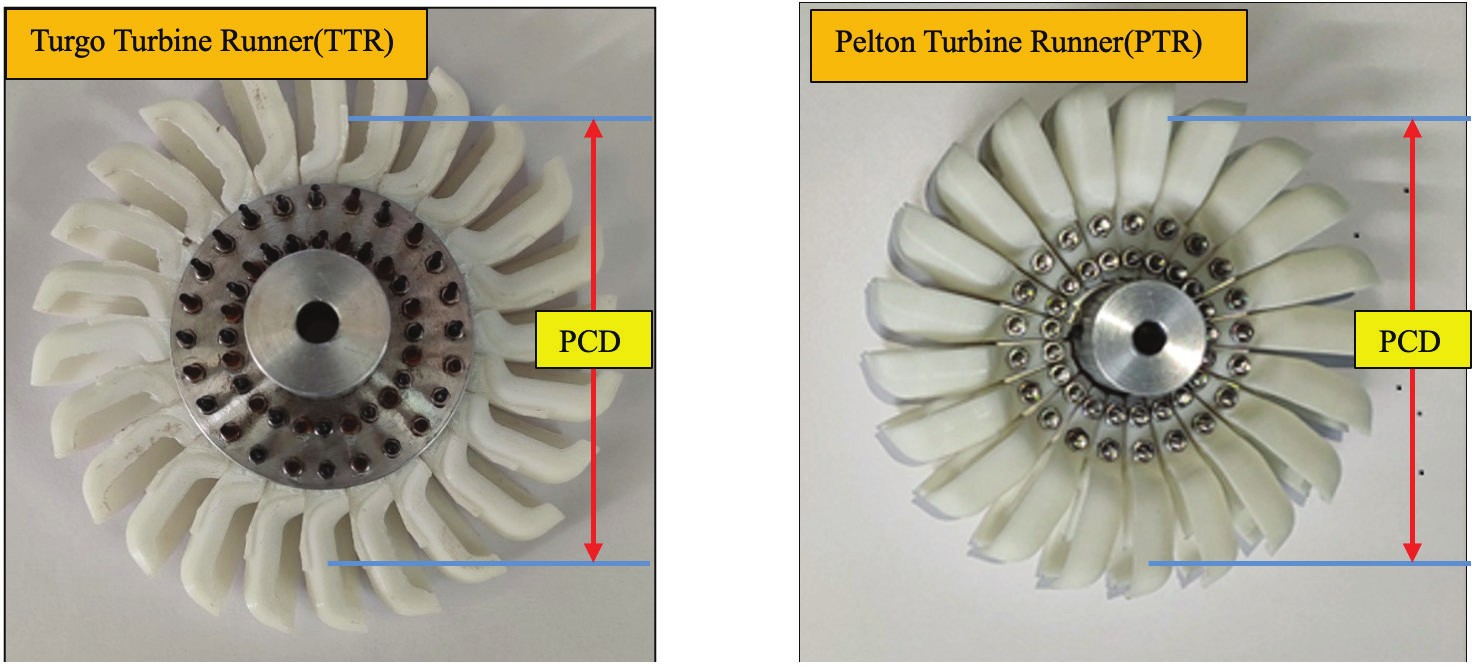
\includegraphics[width=0.85\textwidth]{Figs/lakdawala_rodetes.jpg}
\caption{Las dos turbinas del experimento, Turgo (izquierda) y Pelton (derecha), vistas desde arriba. La flecha roja marca el diámetro de la circunferencia donde el chorro golpea los cangilones, que es el mismo en las dos. Fuente: \citet{Lakdawala2025}.}
\label{fig:rodetes}
\end{figure}

Las turbinas se probaron en el banco de pruebas de la Figura~\ref{fig:montaje}, con la misma altura de agua en todos los ensayos. Una bomba lleva el agua hasta las boquillas, el chorro hace girar la rueda y, en cada ensayo, se midieron el caudal de agua, la velocidad de giro de la rueda y la fuerza de giro en el eje; con esas tres mediciones se calculó la eficiencia. Los detalles técnicos del montaje no son necesarios para el análisis estadístico, pero los términos que aparecen en el artículo original se explican en el glosario del Apéndice~\ref{sec:glosario}.

\begin{figure}[H]
\centering
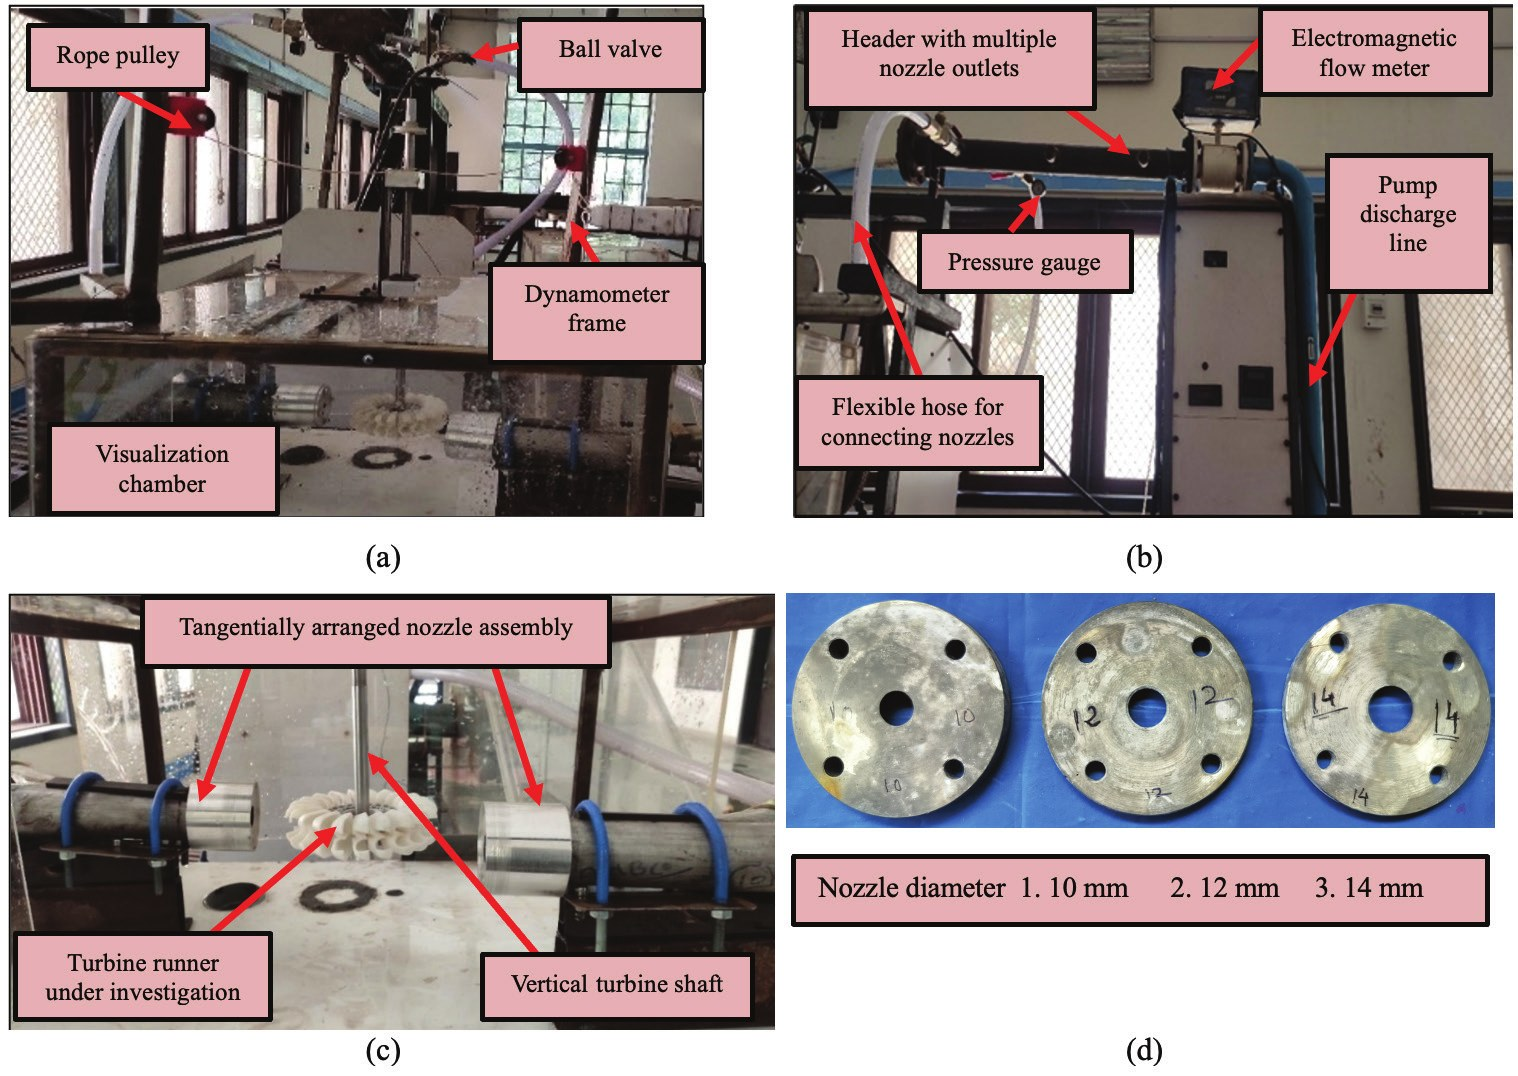
\includegraphics[width=0.9\textwidth]{Figs/lakdawala_montaje.jpg}
\caption{Banco de pruebas: (a) sistema para medir la fuerza de giro en el eje, (b) tubería con el medidor de caudal, (c) las dos boquillas frente a la turbina y (d) las tres placas que fijan el diámetro de la boquilla (10, 12 y 14~mm). Fuente: \citet{Lakdawala2025}.}
\label{fig:montaje}
\end{figure}

En cada uno de los 80 ensayos, llamados corridas, los investigadores fijaron cinco variables: el tipo de turbina (Pelton o Turgo), el número de boquillas (una o dos) y tres características de la boquilla, que son su diámetro (10, 12 o 14~mm), su ángulo y su distancia a la rueda. La Figura~\ref{fig:chorro} muestra qué significan las dos últimas. El ángulo indica qué tan de frente llega el chorro a la rueda: 90° es perpendicular y 92.5° y 95° son desviaciones pequeñas. La distancia es el recorrido del chorro entre la boquilla y la rueda, que se varió entre 40 y 60~mm.

\begin{figure}[H]
\centering
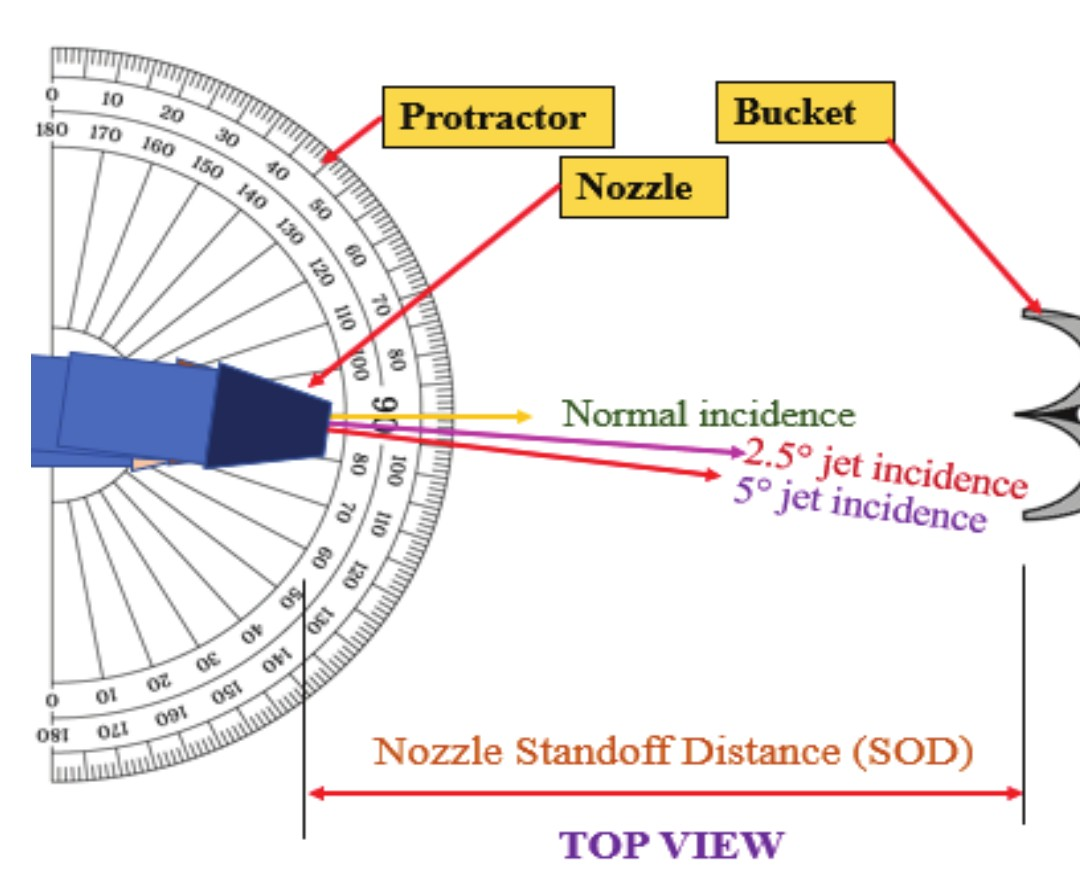
\includegraphics[width=0.55\textwidth]{Figs/lakdawala_chorro.jpg}
\caption{Vista desde arriba de la boquilla y un cangilón: ángulo del chorro (perpendicular, desviado 2.5° y desviado 5°) y distancia entre la boquilla y el cangilón (\textit{Nozzle Standoff Distance}). Fuente: \citet{Lakdawala2025}.}
\label{fig:chorro}
\end{figure}

Las combinaciones de valores no se escogieron al azar. Los autores usaron un diseño central compuesto, un tipo de diseño experimental pensado para ajustar modelos de regresión con términos cuadráticos usando pocas corridas. Por eso cada variable numérica toma solo tres valores (bajo, medio y alto) y varias corridas se repiten en el punto central, con las tres variables en su valor medio. Con estos datos, los autores ajustaron un modelo de regresión cuadrático y buscaron la combinación de variables que maximiza la eficiencia.

En este trabajo se usan los datos publicados por \citet{Lakdawala2025} para estudiar, con las herramientas del análisis de regresión, cómo se relaciona la eficiencia hidráulica con las cinco variables. Primero se presenta el análisis exploratorio de los datos y luego se replica el modelo de regresión reportado por los autores, se verifican sus supuestos y se revisa la condición de máxima eficiencia. Todos los cálculos y gráficos se hicieron en R \citep{RCoreTeam} con los paquetes \textsf{ggplot2} \citep{Wickham2016}, \textsf{GGally} \citep{GGally} y \textsf{car} \citep{Fox2019}, y el código está en el repositorio indicado en la sección de disponibilidad de datos.


\section{Metodología}
\label{sec:metodologia}
% ------------------------------------------------------------
% 2. Metodología
% ------------------------------------------------------------

\subsection{Datos}
\label{sec:datos}

Los datos provienen de la Tabla~6 de \citet{Lakdawala2025} y corresponden a las 80 corridas descritas en la introducción. La variable respuesta es la eficiencia hidráulica, expresada como proporción (entre 0 y 1). La Tabla~\ref{tab:variables} resume las variables y el nombre con el que aparecen en la base de datos.

\begin{table}[ht]
\centering
\caption{Variables del estudio.}
\label{tab:variables}
\begin{tabular}{llll}
\toprule
Variable & Nombre en R & Tipo & Niveles \\
\midrule
Eficiencia hidráulica ($y$)            & \texttt{eficiencia} & Respuesta numérica   & 0.6025 a 0.7165 \\
Ángulo de la boquilla ($\alpha$)       & \texttt{angulo}     & Numérica (grados)    & 90, 92.5, 95 \\
Diámetro de la boquilla ($d_j$)        & \texttt{diametro}   & Numérica (mm)        & 10, 12, 14 \\
Distancia boquilla-rodete ($N_{sod}$)  & \texttt{distancia}  & Numérica (mm)        & 40, 50, 60 \\
Tipo de rodete                         & \texttt{rodete}     & Categórica           & Pelton (PTR), Turgo (TTR) \\
Número de boquillas ($n$)              & \texttt{boquillas}  & Categórica           & 1, 2 \\
\bottomrule
\end{tabular}
\end{table}

Al revisar la Tabla~6 se encontró que en dos corridas los niveles publicados no coinciden con los valores predichos que reportan los mismos autores: en la corrida 12 el ángulo corresponde a 95° (no a 90°) y en la corrida 15 la distancia corresponde a 60~mm (no a 40~mm). En este trabajo se usan esos dos niveles corregidos; con ellos el diseño queda completo y el modelo reproduce exactamente los resultados del artículo.

Los datos y el código del análisis están disponibles en \url{https://github.com/mariasaurius/Articulo_regresion}. El script \texttt{anal\_descrip.R} produce las tablas y figuras del análisis descriptivo, y el script \texttt{mod\_lin.R} las del modelo de regresión. Ambos leen los datos desde el repositorio y aplican la misma corrección.

\subsection{Modelo de regresión}
\label{sec:modelo}

El objetivo es encontrar una ecuación que prediga la eficiencia a partir de las cinco variables. El análisis descriptivo de la Sección~\ref{sec:descriptivo} mostró dos cosas que esa ecuación debe poder representar.

\begin{itemize}
  \item \textbf{Curvatura.} La eficiencia no baja en línea recta cuando aumenta el ángulo. Según la Tabla~\ref{tab:niveles}, la eficiencia media pasa de 0.6813 a 90° a 0.6478 a 92.5° (baja 0.0335) y luego a 0.6389 a 95° (baja solo 0.0089). Los dos pasos son de 2.5°, pero la primera caída es casi cuatro veces la segunda. Si la relación fuera una recta, las dos caídas serían iguales. Con la distancia pasa algo parecido.
  \item \textbf{Interacciones.} El efecto de una variable parece depender de otra; por ejemplo, el diámetro casi no cambia la eficiencia con 90° pero sí con 95° (Tabla~\ref{tab:angulo_diametro}).
\end{itemize}

Un modelo con solo rectas no puede representar ninguna de las dos cosas. Por eso, siguiendo a \citet{Lakdawala2025}, se usa un modelo de segundo orden, que es el modelo típico de la metodología de superficie de respuesta.

\subsubsection{Codificación de las variables}

Antes de ajustar el modelo, las variables se pasan a una escala común. Cada variable numérica se codifica de modo que su nivel bajo valga $-1$, el medio $0$ y el alto $1$, y las dos categóricas se codifican con $+1$ y $-1$. La Tabla~\ref{tab:codificacion} resume las cinco variables codificadas, que se llaman $A$, $B$, $C$, $D$ y $E$, como en el artículo original.

\begin{table}[ht]
\centering
\caption{Codificación de las variables del modelo.}
\label{tab:codificacion}
\small
\begin{tabular}{clllc}
\toprule
Símbolo & Variable & Niveles originales & Fórmula & Codificada \\
\midrule
$A$ & Ángulo de la boquilla     & 90°, 92.5°, 95°    & $(\text{ángulo} - 92.5)/2.5$    & $-1$, $0$, $1$ \\
$B$ & Diámetro de la boquilla   & 10, 12, 14 mm      & $(\text{diámetro} - 12)/2$      & $-1$, $0$, $1$ \\
$C$ & Distancia boquilla-rodete & 40, 50, 60 mm      & $(\text{distancia} - 50)/10$    & $-1$, $0$, $1$ \\
$D$ & Tipo de rodete            & Pelton, Turgo      & Pelton $= +1$, Turgo $= -1$     & $+1$, $-1$ \\
$E$ & Número de boquillas       & 1, 2               & Una $= +1$, dos $= -1$          & $+1$, $-1$ \\
\bottomrule
\end{tabular}
\end{table}

La fórmula de las numéricas resta el valor central y divide por la mitad del rango. Por ejemplo, para el ángulo: $(90 - 92.5)/2.5 = -1$, $(92.5 - 92.5)/2.5 = 0$ y $(95 - 92.5)/2.5 = 1$. La codificación tiene tres ventajas.

\begin{enumerate}
  \item \textbf{Permite comparar el tamaño de los coeficientes.} En las unidades originales, el coeficiente de una variable dice cuánto cambia la eficiencia por cada unidad de esa variable: por cada grado de ángulo o por cada milímetro de distancia. Pero esas unidades no son comparables entre sí: un grado es la quinta parte del rango del ángulo (de 90° a 95°), mientras que un milímetro es apenas la vigésima parte del rango de la distancia (de 40 a 60~mm). Una variable podría tener un coeficiente pequeño solo porque su unidad es pequeña, no porque importe poco. Con la codificación, una unidad es lo mismo para todas las variables: ir del centro al extremo de su rango. Así, el coeficiente más grande en valor absoluto corresponde a la variable que más mueve la eficiencia dentro del experimento.
  \item \textbf{Le da sentido al intercepto.} El intercepto es la predicción cuando todas las variables valen cero. En las unidades originales eso sería un ángulo de 0° y una boquilla de 0~mm, condiciones que no tienen sentido. Con la codificación, $A = B = C = 0$ es el centro del diseño (92.5°, 12~mm y 50~mm), y $D = E = 0$ es el punto medio entre $+1$ y $-1$, es decir, el promedio entre los dos rodetes y entre una y dos boquillas. Por eso el intercepto es la eficiencia predicha en el centro del diseño, promediando rodetes y número de boquillas.
  \item \textbf{Permite comparar con el artículo.} Es la escala que usa el programa Design Expert, con el que los autores ajustaron su modelo.
\end{enumerate}

\subsubsection{El modelo de segundo orden}

La forma general de un modelo de segundo orden con $k$ variables es
\begin{equation}
y = \beta_0 + \sum_{i=1}^{k} \beta_i x_i + \sum_{i=1}^{k} \beta_{ii} x_i^2 + \sum_{i<j} \beta_{ij} x_i x_j + \varepsilon,
\label{eq:general}
\end{equation}
es decir, tiene un intercepto, un término de primer orden para cada variable ($x_i$), un término cuadrático para cada variable ($x_i^2$) y un término de interacción para cada pareja de variables ($x_i x_j$) \citep{Montgomery2005}. Con $k$ variables hay $k$ términos de primer orden, $k$ cuadráticos y $k(k-1)/2$ interacciones; con $k = 5$ serían $1 + 5 + 5 + 10 = 21$ coeficientes.

El modelo de este trabajo tiene 19 y no 21 porque le faltan los cuadrados de $D$ y $E$. Como esas variables solo valen $+1$ o $-1$, su cuadrado siempre es $(+1)^2 = (-1)^2 = 1$: una columna de unos, igual a la del intercepto, que no aporta información nueva. Por eso solo las variables numéricas, que tienen tres niveles, llevan término cuadrático. El modelo queda así:
\begin{align}
y = \beta_0
&+ \underbrace{\beta_1 A + \beta_2 B + \beta_3 C + \beta_4 D + \beta_5 E}_{\text{5 efectos principales}}
 + \underbrace{\beta_{11} A^2 + \beta_{22} B^2 + \beta_{33} C^2}_{\text{3 términos cuadráticos}} \nonumber \\
&+ \underbrace{\beta_{12} AB + \beta_{13} AC + \cdots + \beta_{45} DE}_{\text{10 interacciones dobles}}
 + \varepsilon, \qquad \varepsilon \sim N(0, \sigma^2),
\label{eq:modelo2}
\end{align}
con $1 + 5 + 3 + 10 = 19$ coeficientes. Cada grupo de términos cumple una función:
\begin{itemize}
  \item \textbf{Intercepto} ($\beta_0$): la eficiencia predicha en el centro del diseño, como se explicó arriba.
  \item \textbf{Efectos principales} ($\beta_1, \ldots, \beta_5$): el efecto de cada variable por sí sola, con las demás en el centro. Como cada variable va de $-1$ a $1$, su coeficiente es la mitad de la diferencia entre la eficiencia predicha en el nivel alto y en el nivel bajo. Por ejemplo, $\beta_1$ es la mitad de la diferencia entre la eficiencia predicha con 95° y con 90°. Si es negativo, la eficiencia es menor en el nivel alto que en el bajo.
  \item \textbf{Términos cuadráticos} ($\beta_{11}, \beta_{22}, \beta_{33}$): permiten que la relación sea una curva y no una recta, es decir, que la caída de $-1$ a $0$ sea distinta de la caída de $0$ a $1$, como pasa con el ángulo.
  \item \textbf{Interacciones dobles} ($\beta_{12}, \ldots, \beta_{45}$): el producto de dos variables permite que el efecto de una dependa del valor de la otra. Con cinco variables hay $5 \times 4 / 2 = 10$ parejas posibles: $AB$, $AC$, $AD$, $AE$, $BC$, $BD$, $BE$, $CD$, $CE$ y $DE$.
\end{itemize}

Aunque la ecuación tiene cuadrados y productos, sigue siendo un modelo de \emph{regresión lineal}. La palabra \emph{lineal} se refiere a los coeficientes $\beta$, no a las variables: la eficiencia es una suma de coeficientes multiplicados por columnas de datos. Una columna como $A^2$ o $AB$ se calcula a partir de los datos antes de ajustar el modelo y, para el método de estimación, es una variable más. Un modelo no lineal sería, por ejemplo, $y = \beta_0 e^{\beta_1 A}$, donde un coeficiente aparece dentro de una exponencial.

\subsubsection{La matriz de diseño}

Escrito en forma matricial, el modelo es $\mathbf{y} = \mathbf{X}\bm{\beta} + \bm{\varepsilon}$, donde $\mathbf{y}$ tiene las 80 eficiencias, $\bm{\beta}$ los 19 coeficientes y $\mathbf{X}$ es la matriz de diseño, con una fila por corrida y una columna por coeficiente. La Tabla~\ref{tab:matrizX} muestra cuatro filas de $\mathbf{X}$ (sección~5.1 de \texttt{mod\_lin.R}). La primera columna es de unos (para el intercepto); las cinco siguientes son las variables codificadas, y las demás se obtienen elevando al cuadrado o multiplicando esas columnas. Por ejemplo, en la corrida~2 ($A = -1$, $B = 1$) la columna $AB$ vale $(-1)(1) = -1$, y en la corrida~5, que está en el centro del diseño, todas las columnas que contienen $A$, $B$ o $C$ valen cero.

\begin{table}[ht]
\centering
\caption{Cuatro filas de la matriz de diseño $\mathbf{X}$: corrida 1 (95°, 12~mm, 50~mm, Pelton, dos boquillas), corrida 2 (90°, 14~mm, 40~mm, Turgo, una boquilla), corrida 5 (punto central, Turgo, dos boquillas) y corrida 11 (90°, 10~mm, 40~mm, Turgo, dos boquillas).}
\label{tab:matrizX}
\setlength{\tabcolsep}{2.6pt}
\footnotesize
\begin{tabular}{c|r|rrrrr|rrr|rrrrrrrrrr}
\toprule
Corr. & 1 & $A$ & $B$ & $C$ & $D$ & $E$ & $A^2$ & $B^2$ & $C^2$ & $AB$ & $AC$ & $AD$ & $AE$ & $BC$ & $BD$ & $BE$ & $CD$ & $CE$ & $DE$ \\
\midrule
1  & 1 &  1 &  0 &  0 &  1 & $-1$ & 1 & 0 & 0 &  0 & 0 & 1 & $-1$ &  0 &  0 & 0 & 0 &  0 & $-1$ \\
2  & 1 & $-1$ &  1 & $-1$ & $-1$ &  1 & 1 & 1 & 1 & $-1$ & 1 & 1 & $-1$ & $-1$ & $-1$ & 1 & 1 & $-1$ & $-1$ \\
5  & 1 &  0 &  0 &  0 & $-1$ & $-1$ & 0 & 0 & 0 &  0 & 0 & 0 &  0 &  0 &  0 & 0 & 0 &  0 &  1 \\
11 & 1 & $-1$ & $-1$ & $-1$ & $-1$ & $-1$ & 1 & 1 & 1 &  1 & 1 & 1 &  1 &  1 &  1 & 1 & 1 &  1 &  1 \\
\bottomrule
\end{tabular}
\end{table}

Los coeficientes se estiman por mínimos cuadrados, $\hat{\bm{\beta}} = (\mathbf{X}^\top\mathbf{X})^{-1}\mathbf{X}^\top\mathbf{y}$, igual que en cualquier regresión lineal múltiple \citep{Montgomery2005}. En R el modelo se ajusta con la función \texttt{lm()}.

\subsubsection{Evaluación del modelo}

La significancia de cada término se evalúa con un análisis de varianza (ANOVA) con sumas de cuadrados tipo III, como en el artículo original. Para entender por qué se usa esta, conviene compararla con la suma de cuadrados tipo I, que es la que da la función \texttt{anova()} de R. La tipo I agrega los términos uno por uno, en el orden en que están escritos en la fórmula, y a cada término le asigna lo que reduce el error \emph{en el momento en que entra}. Si dos términos explican en parte lo mismo, el que entra primero se queda con esa parte y el que entra después recibe solo lo que agrega de nuevo; al cambiar el orden, cambian los resultados. Es como repartir el mérito de un trabajo en grupo según quién habló primero.

La tipo III evita ese problema. A cada término le asigna lo que reduce el error cuando se agrega a un modelo que ya tiene \emph{todos} los demás términos, es decir, solo lo que ese término explica y ningún otro puede explicar. Como cada término se compara siempre con el mismo conjunto (todos los demás), no importa el orden en que se escriban. Se calculó con la función \texttt{Anova()} del paquete \textsf{car} \citep{Fox2019}.

Además se usan las siguientes medidas:
\begin{itemize}
  \item \textbf{Prueba de falta de ajuste.} Las corridas repetidas en el punto central tienen exactamente las mismas condiciones, así que sus diferencias solo pueden deberse al ruido del experimento; esa variación se llama \emph{error puro}. La prueba compara el error del modelo con el error puro: si el modelo deja sin explicar mucho más que el ruido, su forma no es adecuada.
  \item \textbf{$R^2$ y $R^2$ ajustado.} La proporción de la variabilidad de la eficiencia que explica el modelo; el ajustado penaliza el número de términos.
  \item \textbf{$R^2$ predicho y PRESS.} El PRESS suma los errores que se cometen al predecir cada corrida con un modelo ajustado \emph{sin} esa corrida. Con él se calcula el $R^2$ predicho, que mide qué tan bien predice el modelo datos que no usó para ajustarse.
  \item \textbf{Desviación estándar ($s$) y coeficiente de variación.} El tamaño típico de los errores del modelo, en unidades de eficiencia y como porcentaje de la eficiencia media.
\end{itemize}

Los supuestos del modelo (errores normales, con varianza constante e independientes) se revisan con los residuales estudentizados. Un residual estudentizado es el residual dividido por una estimación de su desviación estándar, de modo que todos quedan en una escala comparable, parecida a la de una normal estándar. El internamente estudentizado usa la desviación estándar del modelo completo; el externamente estudentizado usa la de un modelo ajustado sin esa corrida, para que una corrida atípica no afecte la escala con la que se juzga a sí misma.


\section{Resultados}
\label{sec:resultados}
% ------------------------------------------------------------
% 3. Resultados
% ------------------------------------------------------------

\subsection{Análisis descriptivo}
\label{sec:descriptivo}

\subsubsection{Distribución de la eficiencia hidráulica}

La Tabla~\ref{tab:resumen_y} resume la eficiencia hidráulica de las 80 corridas (sección~4 del script). La eficiencia media es de 0.6540, con una desviación estándar de 0.0245 y un coeficiente de variación de 3.74\,\%, es decir, las eficiencias cambian poco en términos relativos. Los valores van de 0.6025 a 0.7165.

Además de la media y la desviación estándar, la tabla incluye tres medidas de la forma de la distribución:

\begin{itemize}
  \item \textbf{Rango intercuartílico (RIQ).} Es la diferencia entre el tercer cuartil ($Q_3$, el valor que deja por debajo al 75\,\% de los datos) y el primer cuartil ($Q_1$, que deja por debajo al 25\,\%): $\text{RIQ} = Q_3 - Q_1$. Mide la amplitud del 50\,\% central de los datos y, a diferencia del rango o la desviación estándar, no se ve afectado por valores extremos. Aquí $Q_1 = 0.6360$ y $Q_3 = 0.6715$, así que la mitad central de las corridas tiene eficiencias en un intervalo de apenas 0.0355.

  \item \textbf{Asimetría.} Mide si la distribución se extiende más hacia un lado que hacia el otro. Se calcula como
  \[
  g_1 = \frac{\frac{1}{n}\sum_{i=1}^{n}(y_i-\bar{y})^3}{s^3}.
  \]
  Vale cero en una distribución simétrica, es positiva cuando la cola derecha es más larga (hay algunos valores altos alejados del resto) y negativa cuando la cola larga está a la izquierda. El valor de 0.380 indica una asimetría leve hacia la derecha: hay algunas corridas con eficiencias altas, cercanas a 0.70, más alejadas de la media que las corridas de eficiencia baja. Por eso la media (0.6540) queda un poco por encima de la mediana (0.6515).

  \item \textbf{Exceso de curtosis.} La curtosis mide qué tan pesadas son las colas de una distribución, es decir, qué tanto pesan los valores muy alejados de la media. Se calcula como $\frac{1}{n}\sum_{i=1}^{n}(y_i-\bar{y})^4 / s^4$, y en una distribución normal vale 3. Por eso se suele reportar el \emph{exceso} de curtosis, que es la curtosis menos 3, de modo que la normal sirva de referencia con un valor de cero. Un exceso positivo indica colas más pesadas que la normal (más valores extremos de lo esperado) y uno negativo, colas más livianas. El valor de $-0.351$ indica que las eficiencias tienen colas algo más livianas que una normal: hay pocos valores muy alejados de la media.
\end{itemize}

\begin{table}[ht]
\centering
\caption{Medidas descriptivas de la eficiencia hidráulica ($n = 80$).}
\label{tab:resumen_y}
\begin{tabular}{lc@{\hspace{1.5cm}}lc}
\toprule
Medida & Valor & Medida & Valor \\
\midrule
Media               & 0.6540 & Mínimo                  & 0.6025 \\
Mediana             & 0.6515 & Máximo                  & 0.7165 \\
Desviación estándar & 0.0245 & Rango intercuartílico   & 0.0355 \\
Coef. de variación  & 3.74\,\% & Asimetría             & 0.380 \\
                    &        & Exceso de curtosis      & $-0.351$ \\
\bottomrule
\end{tabular}
\end{table}

La Figura~\ref{fig:distribucion} muestra estas características de forma gráfica. El panel~(a) es un histograma: el rango de eficiencias se divide en 12 intervalos y la altura de cada barra indica cuántas corridas caen en ese intervalo, en escala de densidad (el área total de las barras suma uno). La curva negra es una estimación suavizada de esa densidad y la línea roja discontinua marca la media. Se ve una distribución con un solo pico, alrededor de 0.65, y una cola derecha un poco más larga, lo que coincide con la asimetría positiva.

El panel~(b) es un diagrama de caja. La caja va del primer al tercer cuartil ($Q_1 = 0.6360$ y $Q_3 = 0.6715$), así que su altura es el rango intercuartílico y contiene al 50\,\% central de las corridas; la línea negra dentro de la caja es la mediana. Los bigotes se extienden hasta la corrida más extrema que esté a menos de $1.5 \times \text{RIQ}$ de la caja, es decir, entre 0.5828 y 0.7248; los valores por fuera de esos límites se considerarían atípicos. Los puntos negros son las 80 corridas, separadas un poco en horizontal para que no se superpongan. Ninguna corrida queda por fuera de los bigotes, así que no hay eficiencias atípicas, y la mediana está algo más cerca del borde inferior de la caja, otra señal de la leve asimetría a la derecha.

\begin{figure}[ht]
\centering
\begin{minipage}[b]{0.62\textwidth}
  \centering
  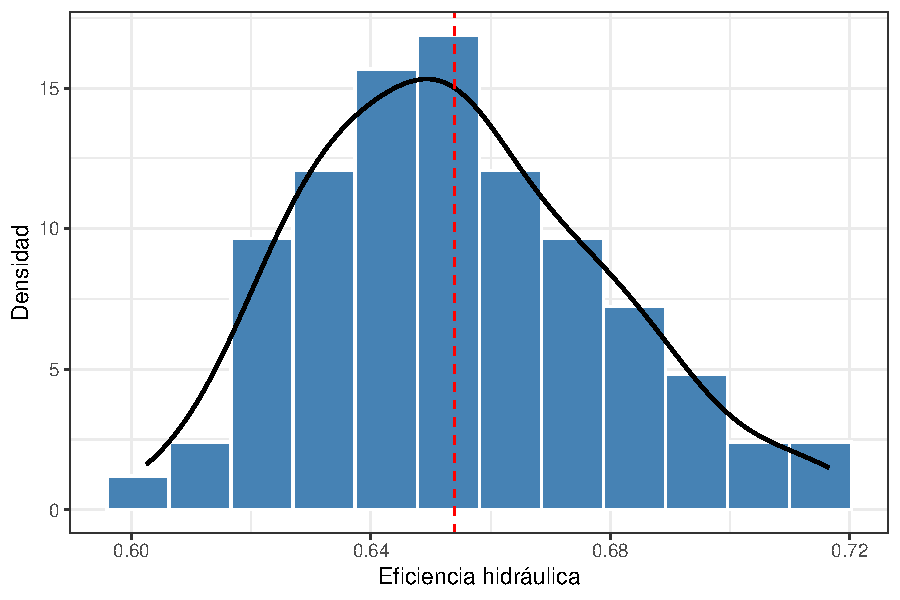
\includegraphics[width=\textwidth]{Articulo_Revista/Figs/g1_histograma.pdf}\\[-2pt]
  {\small (a)}
\end{minipage}\hfill
\begin{minipage}[b]{0.35\textwidth}
  \centering
  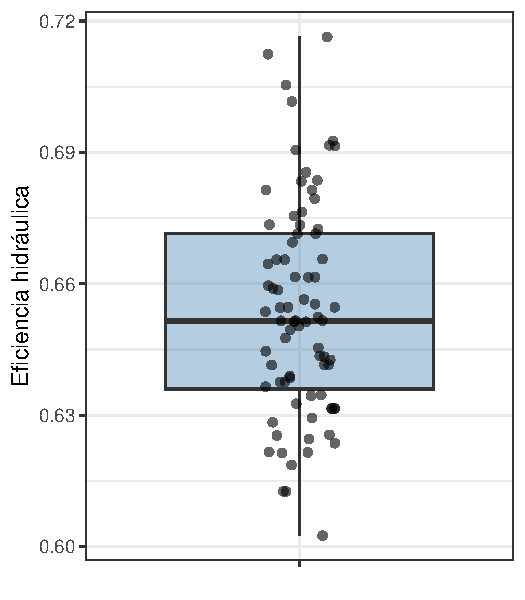
\includegraphics[width=\textwidth]{Articulo_Revista/Figs/g2_boxplot.pdf}\\[-2pt]
  {\small (b)}
\end{minipage}
\caption{Histograma con curva de densidad (a) y diagrama de caja (b) de la eficiencia hidráulica. La línea roja discontinua marca la media. Código: sección~4 de \texttt{anal\_descrip.R}.}
\label{fig:distribucion}
\end{figure}

\subsubsection{Eficiencia según cada variable explicativa}

La Tabla~\ref{tab:niveles} y la Figura~\ref{fig:por_variable} muestran la eficiencia según cada variable explicativa (sección~5 del script). En la figura hay un diagrama de caja por cada nivel de cada variable, construido igual que en la Figura~\ref{fig:distribucion}(b) pero solo con las corridas de ese nivel; los puntos azules son las corridas y el rombo rojo es la media del grupo. Si las cajas de los distintos niveles están a alturas diferentes, la variable está asociada con la eficiencia; si se superponen mucho, la diferencia entre niveles es pequeña comparada con la variación dentro de cada nivel. Los niveles medios (92.5°, 12~mm y 50~mm) tienen el doble de corridas que los extremos porque ahí están las réplicas del punto central.

\begin{table}[ht]
\centering
\caption{Eficiencia hidráulica según el nivel de cada variable explicativa.}
\label{tab:niveles}
\begin{tabular}{llccccc}
\toprule
Variable & Nivel & $n$ & Media & Desv. est. & Mínimo & Máximo \\
\midrule
\multirow{3}{*}{Ángulo (°)}       & 90    & 20 & 0.6813 & 0.0191 & 0.6455 & 0.7165 \\
                                  & 92.5  & 40 & 0.6478 & 0.0171 & 0.6185 & 0.6915 \\
                                  & 95    & 20 & 0.6389 & 0.0204 & 0.6025 & 0.6835 \\
\midrule
\multirow{3}{*}{Diámetro (mm)}    & 10    & 20 & 0.6618 & 0.0271 & 0.6125 & 0.7165 \\
                                  & 12    & 40 & 0.6507 & 0.0193 & 0.6215 & 0.7055 \\
                                  & 14    & 20 & 0.6527 & 0.0300 & 0.6025 & 0.7125 \\
\midrule
\multirow{3}{*}{Distancia (mm)}   & 40    & 20 & 0.6692 & 0.0260 & 0.6255 & 0.7165 \\
                                  & 50    & 40 & 0.6492 & 0.0188 & 0.6185 & 0.7055 \\
                                  & 60    & 20 & 0.6482 & 0.0275 & 0.6025 & 0.7015 \\
\midrule
\multirow{2}{*}{Rodete}           & Pelton & 40 & 0.6441 & 0.0212 & 0.6025 & 0.6925 \\
                                  & Turgo  & 40 & 0.6638 & 0.0238 & 0.6125 & 0.7165 \\
\midrule
\multirow{2}{*}{Boquillas}        & 1     & 40 & 0.6429 & 0.0211 & 0.6025 & 0.6915 \\
                                  & 2     & 40 & 0.6650 & 0.0227 & 0.6235 & 0.7165 \\
\bottomrule
\end{tabular}
\end{table}

El ángulo de la boquilla es la variable con el efecto más claro: la eficiencia media baja de 0.681 a 90° a 0.639 a 95°, y la caja de 90° está por completo por encima de las otras dos. El rodete Turgo es en promedio más eficiente que el Pelton (0.664 frente a 0.644) y usar dos boquillas también aumenta la eficiencia media (0.665 frente a 0.643); en ambos casos las cajas se desplazan hacia arriba, aunque se superponen en parte. Con el diámetro y la distancia la eficiencia media es mayor en el nivel bajo (10~mm y 40~mm), pero las diferencias son menores y las cajas se superponen mucho, porque la dispersión dentro de cada nivel es grande.

\begin{figure}[ht]
\centering
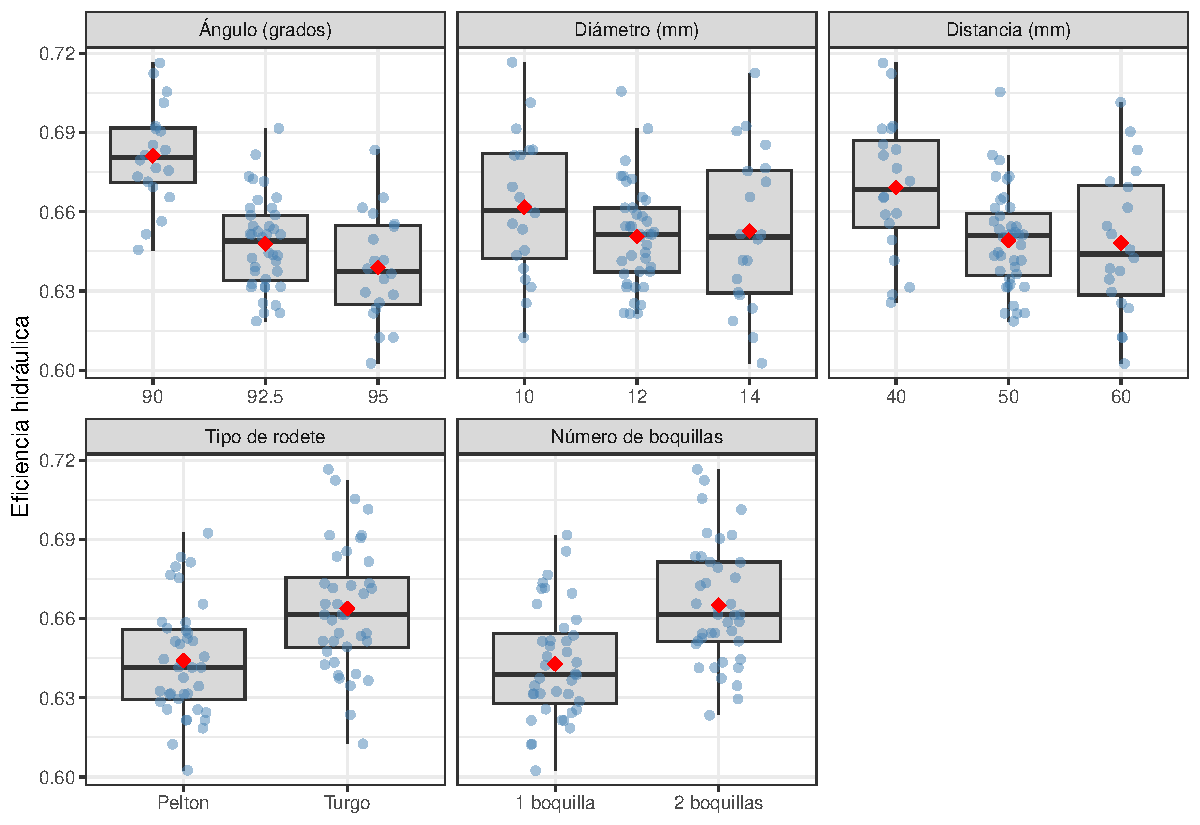
\includegraphics[width=0.92\textwidth]{Articulo_Revista/Figs/g3_boxplot_por_variable.pdf}
\caption{Eficiencia hidráulica según cada variable explicativa. Los rombos rojos marcan la media de cada grupo. Código: sección~5 de \texttt{anal\_descrip.R}.}
\label{fig:por_variable}
\end{figure}

\subsubsection{Eficiencia media con intervalos de confianza}

Los diagramas de caja muestran cómo se reparten las corridas; para comparar los niveles conviene mirar también qué tan precisa es cada media. La Figura~\ref{fig:medias} muestra la eficiencia media de cada nivel con su intervalo de confianza del 95\,\%, calculado con la distribución $t$ de Student:
\[
\bar{y} \pm t_{0.975,\,n-1}\,\frac{s}{\sqrt{n}},
\]
donde $\bar{y}$, $s$ y $n$ son la media, la desviación estándar y el número de corridas del nivel. Cada punto es una media, las barras son el intervalo y la línea une las medias para mostrar la tendencia. La Tabla~\ref{tab:ic} presenta los mismos intervalos (sección~6 del script).

\begin{figure}[ht]
\centering
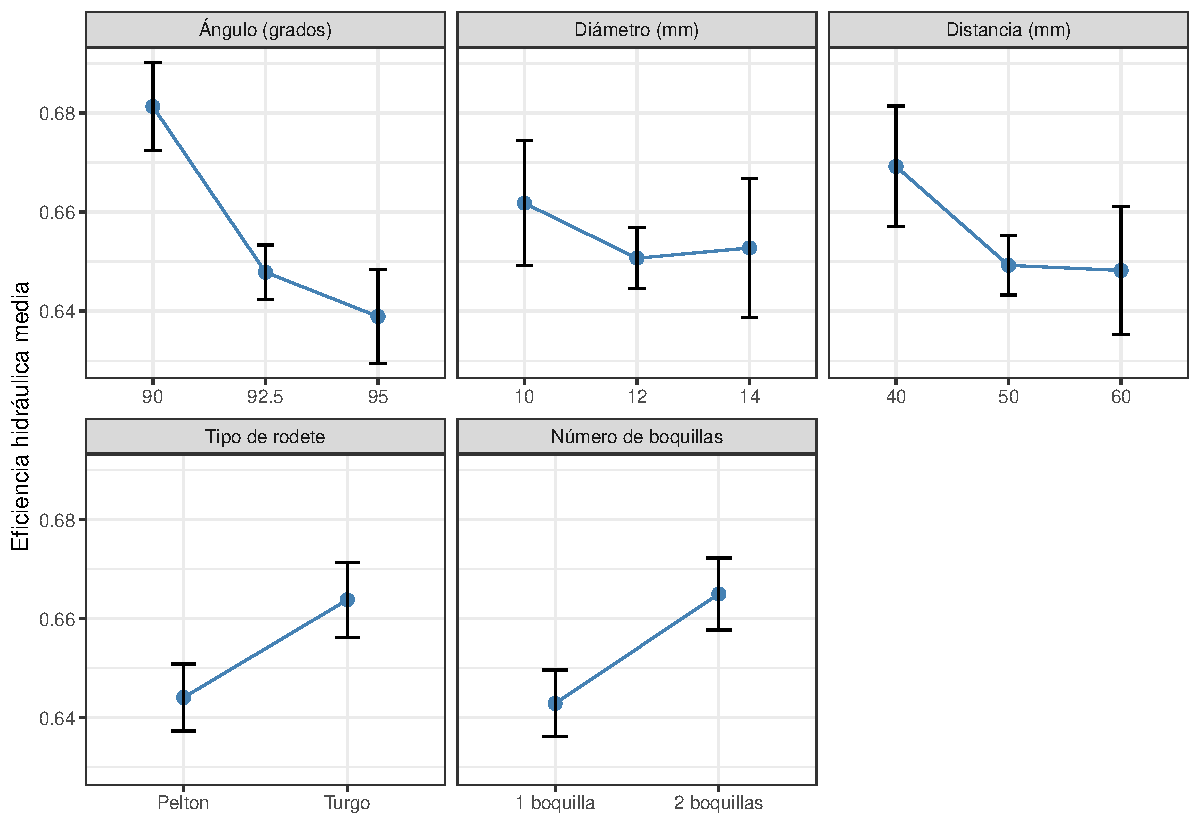
\includegraphics[width=0.92\textwidth]{Articulo_Revista/Figs/g4_medias_ic95.pdf}
\caption{Eficiencia media e intervalo de confianza del 95\,\% para cada nivel de cada variable explicativa. Código: sección~6 de \texttt{anal\_descrip.R}.}
\label{fig:medias}
\end{figure}

\begin{table}[ht]
\centering
\caption{Eficiencia media e intervalo de confianza del 95\,\% por nivel.}
\label{tab:ic}
\begin{tabular}{llcccc}
\toprule
Variable & Nivel & Media & Límite inferior & Límite superior & Ancho \\
\midrule
\multirow{3}{*}{Ángulo (°)}     & 90     & 0.6813 & 0.6724 & 0.6902 & 0.0178 \\
                                & 92.5   & 0.6478 & 0.6424 & 0.6533 & 0.0109 \\
                                & 95     & 0.6389 & 0.6293 & 0.6485 & 0.0192 \\
\midrule
\multirow{3}{*}{Diámetro (mm)}  & 10     & 0.6618 & 0.6491 & 0.6745 & 0.0254 \\
                                & 12     & 0.6507 & 0.6445 & 0.6569 & 0.0124 \\
                                & 14     & 0.6527 & 0.6387 & 0.6668 & 0.0281 \\
\midrule
\multirow{3}{*}{Distancia (mm)} & 40     & 0.6692 & 0.6570 & 0.6814 & 0.0244 \\
                                & 50     & 0.6492 & 0.6432 & 0.6553 & 0.0121 \\
                                & 60     & 0.6482 & 0.6353 & 0.6611 & 0.0258 \\
\midrule
\multirow{2}{*}{Rodete}         & Pelton & 0.6441 & 0.6373 & 0.6509 & 0.0136 \\
                                & Turgo  & 0.6638 & 0.6562 & 0.6714 & 0.0152 \\
\midrule
\multirow{2}{*}{Boquillas}      & 1      & 0.6429 & 0.6362 & 0.6497 & 0.0135 \\
                                & 2      & 0.6650 & 0.6578 & 0.6723 & 0.0145 \\
\bottomrule
\end{tabular}
\end{table}

Una forma informal de leer la figura es fijarse si los intervalos de dos niveles se superponen. Con el ángulo, el intervalo de 90° $[0.6724;\ 0.6902]$ queda completamente por encima de los de 92.5° y 95°, mientras que estos dos últimos se superponen, así que la caída fuerte ocurre entre 90° y 92.5°. Con el tipo de rodete y el número de boquillas los intervalos no se superponen: el Turgo y el uso de dos boquillas tienen una eficiencia media claramente mayor. Con la distancia, el intervalo de 40~mm apenas queda por encima del de 50~mm (0.6570 frente a 0.6553) y se superpone con el de 60~mm. Con el diámetro, los tres intervalos se superponen, de modo que estos datos no muestran por sí solos una diferencia clara entre diámetros.

Los intervalos de los niveles medios son más angostos (alrededor de 0.011 a 0.012, frente a 0.018 a 0.028 en los extremos) porque tienen el doble de corridas y el ancho del intervalo decrece con $\sqrt{n}$. Hay que tener en cuenta dos cosas al interpretar esta figura. Primero, cada media promedia sobre todos los valores de las demás variables, así que no aísla el efecto de una variable manteniendo las otras fijas; eso lo hace el modelo de regresión. Segundo, que dos intervalos se superpongan no prueba que las medias sean iguales: es solo una guía visual, y la comparación formal se hará con las pruebas del modelo.

\subsubsection{Posibles interacciones}

La Figura~\ref{fig:perfiles} presenta gráficos de perfiles (sección~7 del script). Cada línea corresponde a una combinación de tipo de rodete y número de boquillas, y cada punto es la eficiencia media de las corridas de esa combinación en un nivel de la variable del eje horizontal. Este gráfico sirve para buscar interacciones: si el efecto de una variable es el mismo en todas las combinaciones, las líneas son paralelas y solo se desplazan hacia arriba o hacia abajo; si las líneas tienen pendientes distintas o se cruzan, el efecto de esa variable depende del tipo de rodete o del número de boquillas.

\begin{figure}[ht]
\centering
\begin{minipage}[b]{0.49\textwidth}
  \centering
  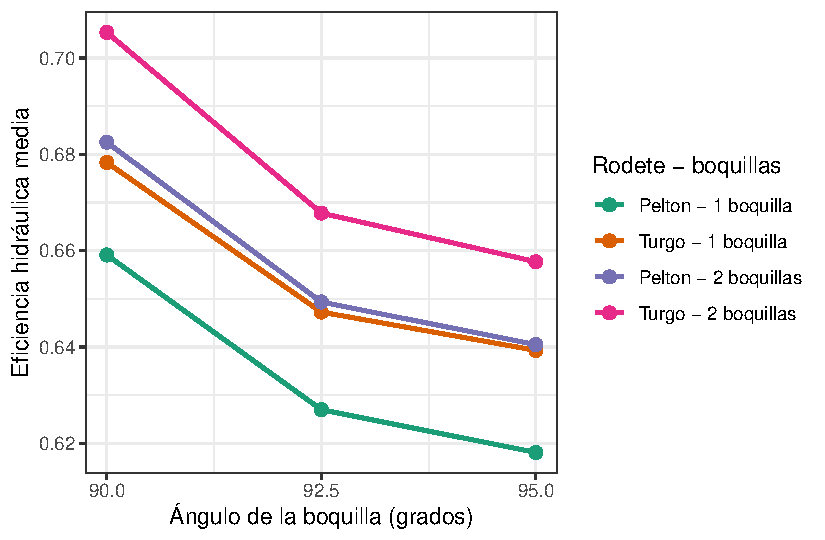
\includegraphics[width=\textwidth]{Articulo_Revista/Figs/perfil_angulo.pdf}\\[-2pt]
  {\small (a)}
\end{minipage}\hfill
\begin{minipage}[b]{0.49\textwidth}
  \centering
  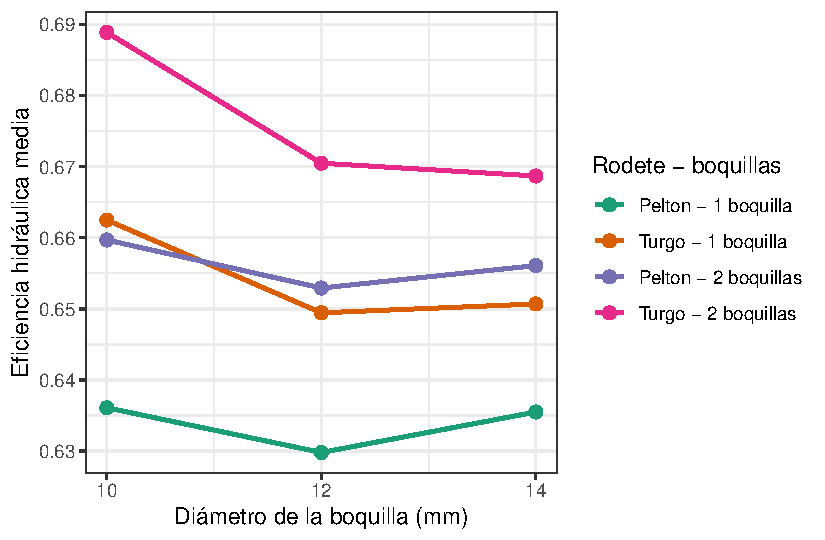
\includegraphics[width=\textwidth]{Articulo_Revista/Figs/perfil_diametro.pdf}\\[-2pt]
  {\small (b)}
\end{minipage}\\[6pt]
\begin{minipage}[b]{0.49\textwidth}
  \centering
  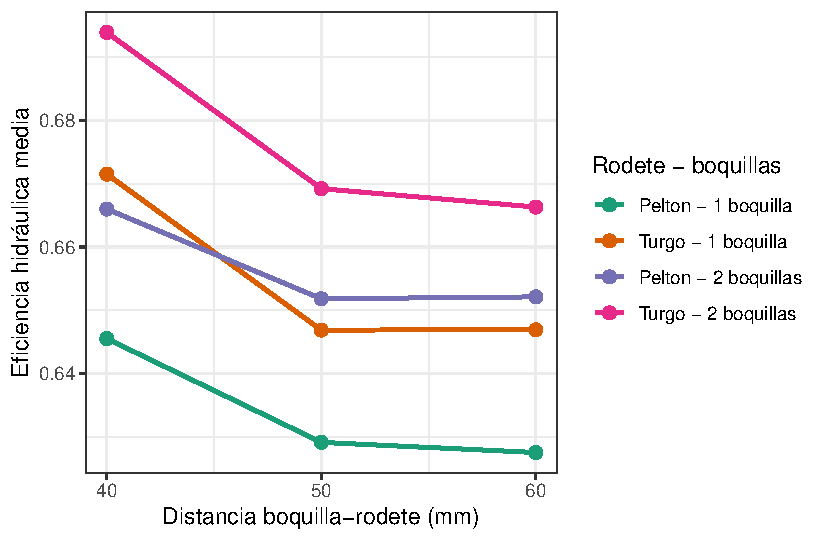
\includegraphics[width=\textwidth]{Articulo_Revista/Figs/perfil_distancia.pdf}\\[-2pt]
  {\small (c)}
\end{minipage}
\caption{Perfiles de la eficiencia media según el ángulo (a), el diámetro (b) y la distancia (c), para cada combinación de tipo de rodete y número de boquillas. Código: sección~7 de \texttt{anal\_descrip.R}.}
\label{fig:perfiles}
\end{figure}

Se ven tres cosas. Primero, la separación vertical entre las líneas confirma los efectos del tipo de rodete y del número de boquillas: el Turgo con dos boquillas va siempre por encima (por ejemplo, 0.7053 a 90°) y el Pelton con una boquilla siempre por debajo (0.6591 a 90°), mientras que el Turgo con una boquilla y el Pelton con dos quedan casi superpuestos en la mitad. Segundo, con el ángulo y con la distancia la eficiencia cae más del nivel bajo al nivel medio que del nivel medio al alto (en el Pelton con una boquilla, por ejemplo, pasa de 0.6591 a 0.6270 y luego a 0.6181 con el ángulo), lo que sugiere curvatura y justifica probar términos cuadráticos. Tercero, las líneas son aproximadamente paralelas, aunque con algunas diferencias de forma: con el diámetro, el Turgo con dos boquillas baja de 0.6889 a 0.6705 entre 10 y 12~mm, mientras que el Pelton con dos boquillas solo baja de 0.6597 a 0.6529. El ajuste del modelo dirá si esas diferencias corresponden a interacciones significativas.

\subsubsection{Gráfico condicional}

La Figura~\ref{fig:condicional} muestra cada corrida por separado (sección~8 del script). El eje horizontal es el ángulo y el vertical la eficiencia; los cuatro paneles separan el tipo de rodete (columnas) y el número de boquillas (filas), y el color indica el diámetro de la boquilla. Los puntos se movieron un poco en horizontal para que no se tapen entre sí. A diferencia de los gráficos anteriores, que resumen con medias, este permite ver tres variables a la vez sin promediar.

\begin{figure}[ht]
\centering
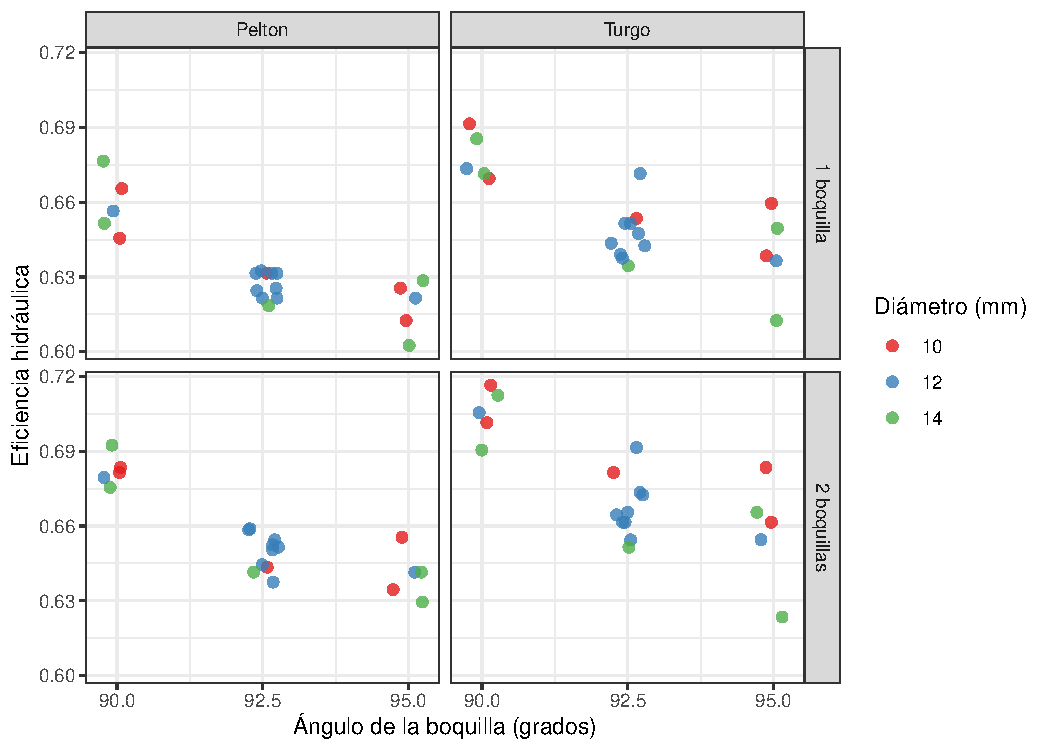
\includegraphics[width=0.85\textwidth]{Articulo_Revista/Figs/g5_condicional.pdf}
\caption{Eficiencia frente al ángulo de la boquilla, por tipo de rodete (columnas) y número de boquillas (filas); el color indica el diámetro. Código: sección~8 de \texttt{anal\_descrip.R}.}
\label{fig:condicional}
\end{figure}

En los cuatro paneles la eficiencia baja al pasar de 90° a 95°, así que el efecto del ángulo se repite en todas las combinaciones de rodete y número de boquillas. Los paneles de la derecha (Turgo) y los de abajo (dos boquillas) están en general más arriba, lo que coincide con lo visto en las medias. El color aporta algo nuevo: con 95° el punto más bajo de cada panel es verde (14~mm), mientras que con 90° los tres colores están mezclados. La Tabla~\ref{tab:angulo_diametro} lo resume con las medias: con 90° la eficiencia media es prácticamente la misma con 10 y con 14~mm (0.6819 y 0.6820), pero con 95° es 0.0148 menor con 14~mm (0.6316 frente a 0.6464). Es decir, el efecto del diámetro parece depender del ángulo, lo que sugiere una posible interacción entre estas dos variables.

\begin{table}[ht]
\centering
\caption{Eficiencia media según el ángulo y el diámetro de la boquilla.}
\label{tab:angulo_diametro}
\begin{tabular}{lccc}
\toprule
 & \multicolumn{3}{c}{Diámetro (mm)} \\
\cmidrule(lr){2-4}
Ángulo (°) & 10 & 12 & 14 \\
\midrule
90   & 0.6819 & 0.6788 & 0.6820 \\
92.5 & 0.6525 & 0.6487 & 0.6365 \\
95   & 0.6464 & 0.6385 & 0.6316 \\
\bottomrule
\end{tabular}
\end{table}

\subsubsection{Correlaciones y matriz de dispersión}

La Tabla~\ref{tab:correlaciones} presenta las correlaciones entre la eficiencia y las variables numéricas (sección~9 del script). La correlación de Pearson mide la fuerza de la relación lineal; la de Spearman se calcula sobre los rangos de los datos y mide si la relación es monótona (siempre creciente o siempre decreciente), aunque no sea una recta. Las tres relaciones son negativas y la del ángulo es la más fuerte, lo que coincide con lo visto en las figuras anteriores. Los dos coeficientes son muy parecidos en las tres variables, lo que indica que las relaciones son monótonas y que no hay valores extremos que distorsionen la correlación de Pearson.

\begin{table}[ht]
\centering
\caption{Correlación de la eficiencia con las variables numéricas.}
\label{tab:correlaciones}
\begin{tabular}{lcc}
\toprule
Variable & Pearson & Spearman \\
\midrule
Ángulo    & $-0.617$ & $-0.593$ \\
Diámetro  & $-0.132$ & $-0.137$ \\
Distancia & $-0.306$ & $-0.288$ \\
\bottomrule
\end{tabular}
\end{table}

La Figura~\ref{fig:matriz} es una matriz de dispersión que reúne todas las variables en un solo gráfico, con el Pelton en verde y el Turgo en naranja. Se lee así:
\begin{itemize}
  \item \textbf{Debajo de la diagonal} están los diagramas de dispersión de cada par de variables. Entre las explicativas los puntos forman una cuadrícula, porque cada una toma solo tres valores fijados por el diseño.
  \item \textbf{En la diagonal} está la densidad de cada variable para cada tipo de rodete. Las de las explicativas son iguales en los dos rodetes, porque ambos se probaron con el mismo diseño; la de la eficiencia del Turgo está corrida hacia la derecha.
  \item \textbf{Encima de la diagonal} está la correlación de cada par, primero para todos los datos (\textit{Corr}) y luego dentro de cada rodete. Los asteriscos indican si la correlación es significativamente distinta de cero: *** para $p < 0.001$, ** para $p < 0.01$, * para $p < 0.05$ y un punto para $p < 0.1$.
  \item \textbf{La última columna} compara cada variable entre los dos rodetes con diagramas de caja, y \textbf{la última fila} muestra los histogramas por rodete.
\end{itemize}

\begin{figure}[ht]
\centering
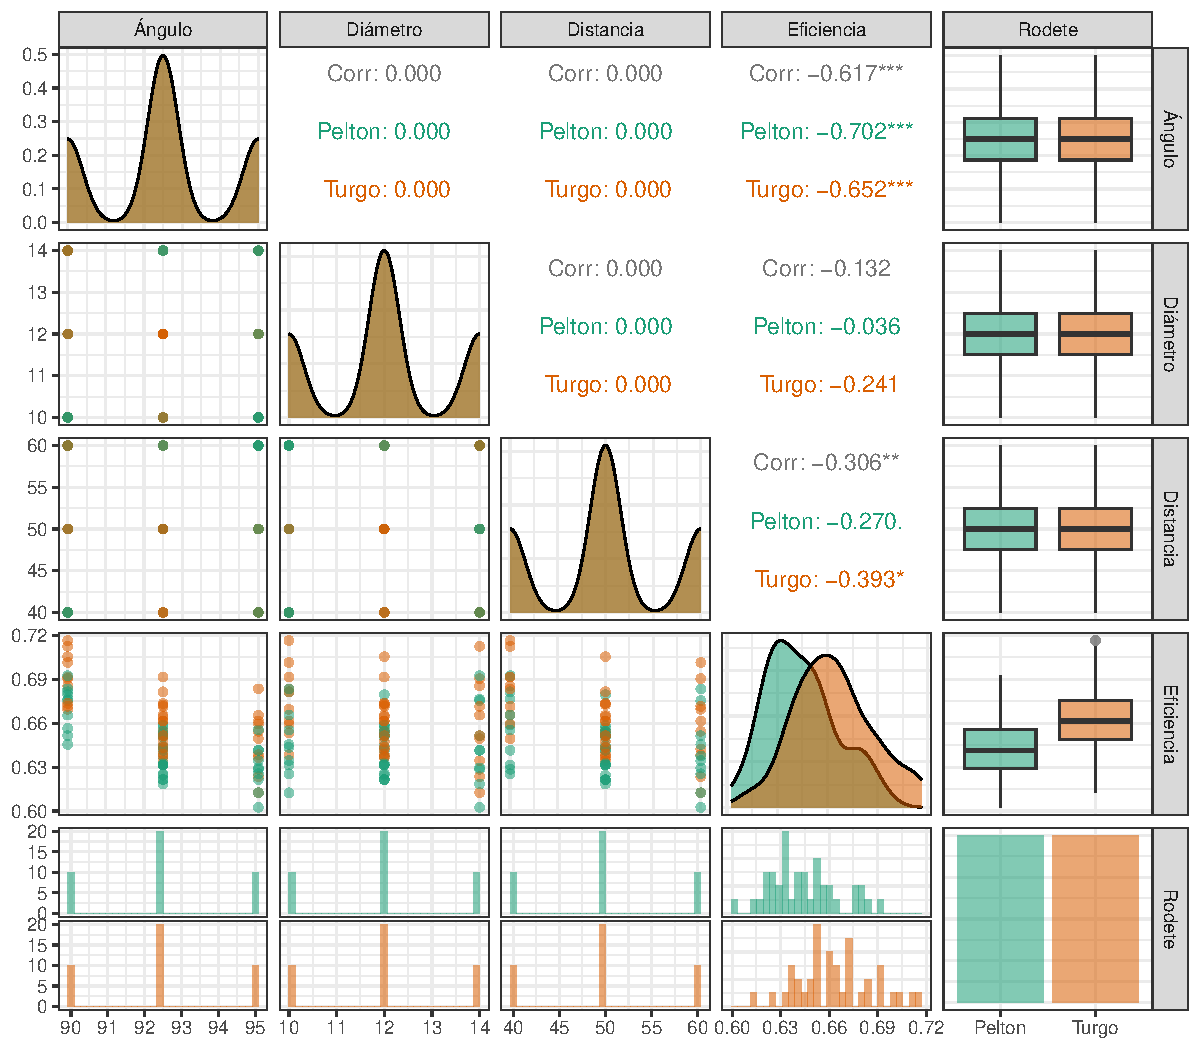
\includegraphics[width=0.9\textwidth]{Articulo_Revista/Figs/g6_matriz_dispersion.pdf}
\caption{Matriz de dispersión de las variables numéricas y del tipo de rodete (verde: Pelton, naranja: Turgo). Código: sección~9 de \texttt{anal\_descrip.R}.}
\label{fig:matriz}
\end{figure}

La información nueva está en las correlaciones dentro de cada rodete. La del ángulo con la eficiencia es de $-0.702$ en el Pelton y $-0.652$ en el Turgo, más fuerte que la total ($-0.617$): al juntar los dos rodetes, la diferencia de nivel entre ellos agrega variación que no tiene que ver con el ángulo y debilita la correlación. La del diámetro es casi nula en el Pelton ($-0.036$) pero de $-0.241$ en el Turgo, y la de la distancia es de $-0.270$ en el Pelton y $-0.393$ en el Turgo. Que la relación del diámetro con la eficiencia cambie según el rodete es otra señal de una posible interacción, en este caso entre el diámetro y el tipo de rodete.

Por último, entre las propias variables explicativas las correlaciones son exactamente cero, tanto con todos los datos como dentro de cada rodete. Es lo que se espera en un diseño experimental, donde los investigadores fijan los valores de cada variable de forma planificada y no dejan que cambien juntas.

% ------------------------------------------------------------
% 3. Resultados: réplica del modelo de regresión (mod_lin.R)
% ------------------------------------------------------------

\subsection{Ajuste del modelo de segundo orden}
\label{sec:ajuste}

La Tabla~\ref{tab:anova_modelo} resume el ANOVA del modelo~\eqref{eq:modelo2} (secciones~6 y~7 de \texttt{mod\_lin.R}). El modelo es significativo ($F = 90.49$ con 18 y 61 grados de libertad, $p < 0.0001$): en conjunto, las variables explican una parte de la variabilidad de la eficiencia mucho mayor que la que se esperaría por azar. La prueba de falta de ajuste no es significativa ($F = 0.97$, $p = 0.5454$): lo que el modelo deja sin explicar es del mismo tamaño que el error puro de las réplicas, así que no hay evidencia de que la forma del modelo sea inadecuada. Estos valores son los mismos de la Tabla~7 de \citet{Lakdawala2025}.

\begin{table}[ht]
\centering
\caption{Análisis de varianza del modelo de segundo orden. SC: suma de cuadrados; gl: grados de libertad; CM: cuadrado medio.}
\label{tab:anova_modelo}
\begin{tabular}{lccccc}
\toprule
Fuente & SC ($\times 10^{-4}$) & gl & CM ($\times 10^{-4}$) & $F$ & Valor $p$ \\
\midrule
Modelo           & 455.93 & 18 & 25.329 & 90.49 & $<0.0001$ \\
Residual         &  17.07 & 61 &  0.280 &       &           \\
\quad Falta de ajuste & 11.37 & 41 & 0.277 & 0.97 & 0.5454 \\
\quad Error puro &   5.70 & 20 &  0.285 &       &           \\
Total            & 473.00 & 79 &       &       &           \\
\bottomrule
\end{tabular}
\end{table}

La Tabla~\ref{tab:coeficientes} presenta los 19 coeficientes estimados, en las variables codificadas, junto con la prueba de cada término (sección~5 de \texttt{mod\_lin.R}). Como cada término tiene un solo grado de libertad, su estadístico $F$ del ANOVA tipo III es el cuadrado de su estadístico $t$, y ambos dan el mismo valor $p$. Al 5\,\% son significativos los cinco efectos principales, las interacciones $AB$, $AC$, $BC$, $BD$ y $CD$ y los términos cuadráticos $A^2$ y $C^2$, exactamente los mismos que reporta el artículo original.

\begin{table}[ht]
\centering
\caption{Coeficientes estimados del modelo en variables codificadas ($A$: ángulo, $B$: diámetro, $C$: distancia, $D$: rodete con Pelton $= +1$, $E$: boquillas con una boquilla $= +1$). EE: error estándar.}
\label{tab:coeficientes}
\begin{tabular}{lrccc}
\toprule
Término & Coeficiente & EE & $F$ & Valor $p$ \\
\midrule
Intercepto & 0.647536 & 0.000909 &        &            \\
$A$        & $-0.021200$ & 0.000837 & 642.26 & $<0.0001$ \\
$B$        & $-0.004525$ & 0.000837 &  29.26 & $<0.0001$ \\
$C$        & $-0.010510$ & 0.000837 & 157.85 & $<0.0001$ \\
$D$        & $-0.009864$ & 0.000592 & 278.07 & $<0.0001$ \\
$E$        & $-0.011061$ & 0.000592 & 349.69 & $<0.0001$ \\
$A^2$      &  0.011317 & 0.001595 &  50.33 & $<0.0001$ \\
$B^2$      & $-0.002808$ & 0.001595 &   3.10 & 0.0834 \\
$C^2$      &  0.004367 & 0.001595 &   7.49 & 0.0081 \\
$AB$       & $-0.003719$ & 0.000935 &  15.81 & 0.0002 \\
$AC$       & $-0.001906$ & 0.000935 &   4.15 & 0.0459 \\
$AD$       &  0.000450 & 0.000837 &   0.29 & 0.5926 \\
$AE$       &  0.001200 & 0.000837 &   2.06 & 0.1565 \\
$BC$       & $-0.001969$ & 0.000935 &   4.43 & 0.0394 \\
$BD$       &  0.003475 & 0.000837 &  17.26 & 0.0001 \\
$BE$       &  0.001425 & 0.000837 &   2.90 & 0.0936 \\
$CD$       &  0.002540 & 0.000837 &   9.22 & 0.0035 \\
$CE$       & $-0.000140$ & 0.000837 &   0.03 & 0.8676 \\
$DE$       & $-0.000249$ & 0.000592 &   0.18 & 0.6756 \\
\bottomrule
\end{tabular}
\end{table}

Gracias a la codificación, los coeficientes se leen directamente:
\begin{itemize}
  \item \textbf{Ángulo.} Es el efecto más grande en valor absoluto. Junto con su término cuadrático indica que, con las demás variables en el centro, la eficiencia baja $0.021200 + 0.011317 = 0.0325$ al pasar de 90° a 92.5°, y solo $0.021200 - 0.011317 = 0.0099$ al pasar de 92.5° a 95°. Es la misma curvatura que mostraron las medias descriptivas.
  \item \textbf{Tipo de rodete y número de boquillas.} Con la codificación $\pm 1$, el coeficiente es la distancia de cada nivel al promedio de los dos. El coeficiente de $D$ ($-0.009864$) indica que el Pelton queda 0.0099 por debajo del promedio y el Turgo 0.0099 por encima, una diferencia de $2 \times 0.009864 = 0.0197$ a favor del Turgo. Del mismo modo, usar dos boquillas aumenta la eficiencia en $2 \times 0.011061 = 0.0221$. Estas diferencias coinciden con las de las medias de la Tabla~\ref{tab:niveles} ($0.6638 - 0.6441$ y $0.6650 - 0.6429$), porque en un diseño balanceado como este los efectos de las variables no se mezclan.
  \item \textbf{Interacciones.} La interacción $AB$ es negativa: el efecto del diámetro es $-0.004525 - 0.003719\,A$, casi nulo con 90° ($A = -1$) y más negativo con 95° ($A = 1$). Es lo que se vio en la Tabla~\ref{tab:angulo_diametro}. La interacción $BD$ es positiva: el diámetro casi no afecta al Pelton ($D = +1$) y sí al Turgo ($D = -1$), como sugerían las correlaciones dentro de cada rodete de la Figura~\ref{fig:matriz}.
\end{itemize}

La Tabla~\ref{tab:estadisticas} muestra las medidas de ajuste (sección~8 de \texttt{mod\_lin.R}). El modelo explica el 96.4\,\% de la variabilidad de la eficiencia. El $R^2$ predicho (0.9375) es muy cercano al ajustado (0.9532), lo que indica que el modelo predice casi igual de bien corridas que no usó para ajustarse; el artículo usa como regla que la diferencia entre ambos sea menor que 0.2. La desviación estándar de los errores, 0.0053, equivale a unas cinco milésimas de eficiencia, menos del 1\,\% de la eficiencia media. Todos los valores coinciden con los Apéndices~A2 y~A3 del artículo original.

\begin{table}[ht]
\centering
\caption{Medidas de ajuste del modelo.}
\label{tab:estadisticas}
\begin{tabular}{lc@{\hspace{1.2cm}}lc}
\toprule
Medida & Valor & Medida & Valor \\
\midrule
$R^2$          & 0.9639 & Desviación estándar ($s$)      & 0.0053 \\
$R^2$ ajustado & 0.9532 & Eficiencia media               & 0.6540 \\
$R^2$ predicho & 0.9375 & Coeficiente de variación (\%)  & 0.81 \\
PRESS          & 0.0030 & Precisión adecuada             & 44.34 \\
\bottomrule
\end{tabular}
\end{table}

La precisión adecuada es una medida que reporta Design Expert: compara el rango de las predicciones con su error típico, y valores mayores que 4 indican que el modelo distingue bien entre condiciones buenas y malas.

\subsection{Ecuaciones para cada tipo de rodete y número de boquillas}

Al fijar el tipo de rodete y el número de boquillas, el modelo queda como una ecuación solo en $A$, $B$ y $C$. Los términos $AB$, $AC$, $BC$, $A^2$, $B^2$ y $C^2$ son los mismos en las cuatro ecuaciones; lo que cambia es el intercepto y los coeficientes de $A$, $B$ y $C$, por las interacciones con $D$ y $E$. La Tabla~\ref{tab:ecuaciones} presenta esos coeficientes (sección~9 de \texttt{mod\_lin.R}), que corresponden a las ecuaciones~(6) a~(9) de \citet{Lakdawala2025}. Todos coinciden con los del artículo excepto uno: el coeficiente de $B$ para el Pelton con dos boquillas aparece en el artículo como $+0.002475$, mientras que el modelo da $-0.002475$. Como el modelo es aditivo en $D$ y $E$, ese coeficiente debe ser igual al del Pelton con una boquilla más el del Turgo con dos menos el del Turgo con una, $0.000375 - 0.009425 + 0.006575 = -0.002475$, lo que indica un error de signo en el artículo.

\begin{table}[ht]
\centering
\caption{Coeficientes de las ecuaciones de cada combinación de rodete y número de boquillas, en variables codificadas. Términos comunes a las cuatro: $-0.003719\,AB - 0.001906\,AC - 0.001969\,BC + 0.011317\,A^2 - 0.002808\,B^2 + 0.004367\,C^2$.}
\label{tab:ecuaciones}
\begin{tabular}{llcrrr}
\toprule
Rodete & Boquillas & Intercepto & $A$ & $B$ & $C$ \\
\midrule
Pelton & 1 & 0.626362 & $-0.019550$ &  0.000375 & $-0.008110$ \\
Pelton & 2 & 0.648982 & $-0.021950$ & $-0.002475$ & $-0.007830$ \\
Turgo  & 1 & 0.646587 & $-0.020450$ & $-0.006575$ & $-0.013190$ \\
Turgo  & 2 & 0.668212 & $-0.022850$ & $-0.009425$ & $-0.012910$ \\
\bottomrule
\end{tabular}
\end{table}

Las cuatro ecuaciones confirman lo anterior: el ángulo tiene el coeficiente más grande en todos los casos, el diámetro casi no influye en el Pelton y sí en el Turgo, y la distancia pesa más en el Turgo ($-0.0132$ y $-0.0129$) que en el Pelton ($-0.0081$ y $-0.0078$).

\subsection{Verificación de los supuestos}

La Figura~\ref{fig:diagnosticos} reproduce los cuatro gráficos de diagnóstico de la Figura~9 del artículo original (sección~10 de \texttt{mod\_lin.R}). En todos, el color de cada punto indica la eficiencia observada en esa corrida.

\begin{figure}[ht]
\centering
\begin{minipage}[b]{0.49\textwidth}
  \centering
  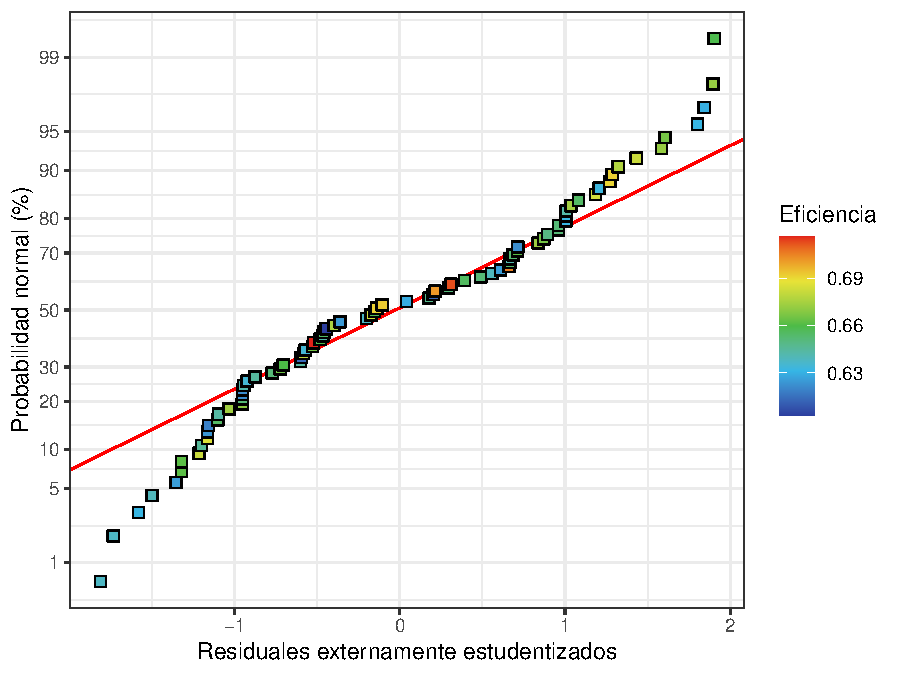
\includegraphics[width=\textwidth]{Articulo_Revista/Figs/fig9a_normal_residuales.pdf}\\
  {\small (a)}
\end{minipage}\hfill
\begin{minipage}[b]{0.49\textwidth}
  \centering
  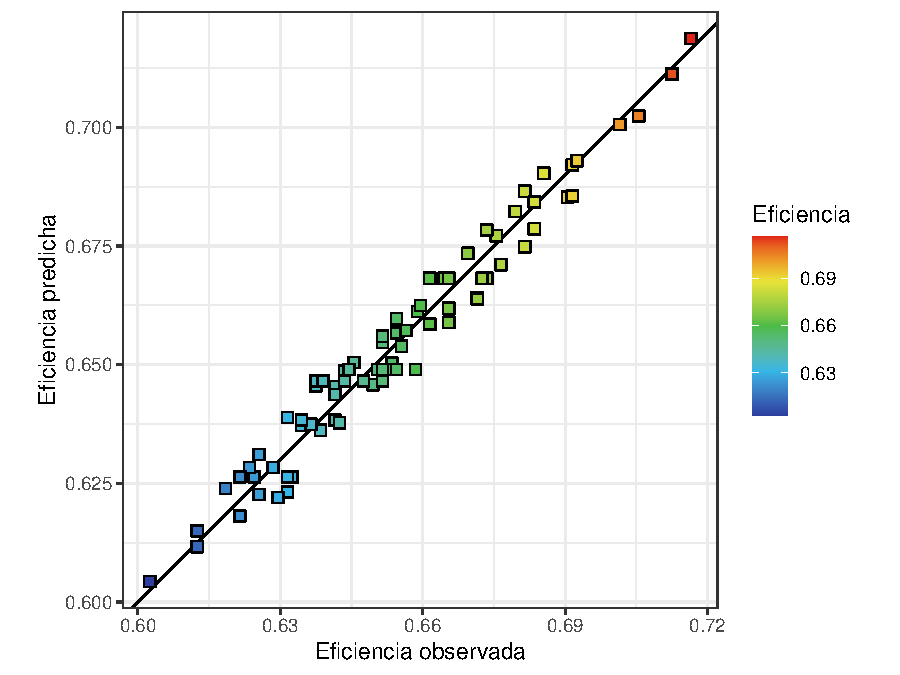
\includegraphics[width=\textwidth]{Articulo_Revista/Figs/fig9b_predicha_observada.pdf}\\
  {\small (b)}
\end{minipage}\\[6pt]
\begin{minipage}[b]{0.49\textwidth}
  \centering
  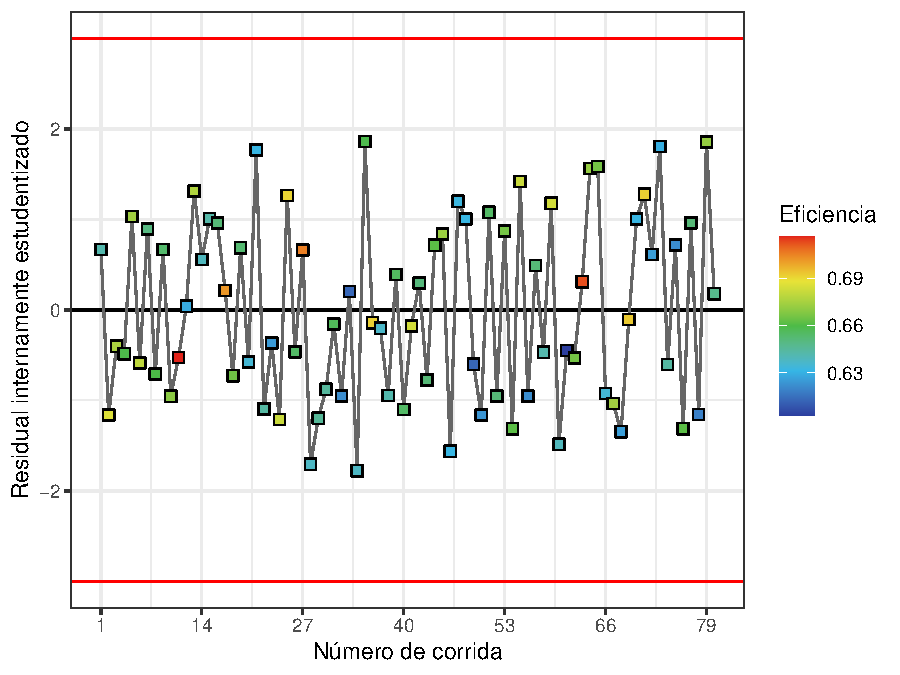
\includegraphics[width=\textwidth]{Articulo_Revista/Figs/fig9c_rint_corrida.pdf}\\
  {\small (c)}
\end{minipage}\hfill
\begin{minipage}[b]{0.49\textwidth}
  \centering
  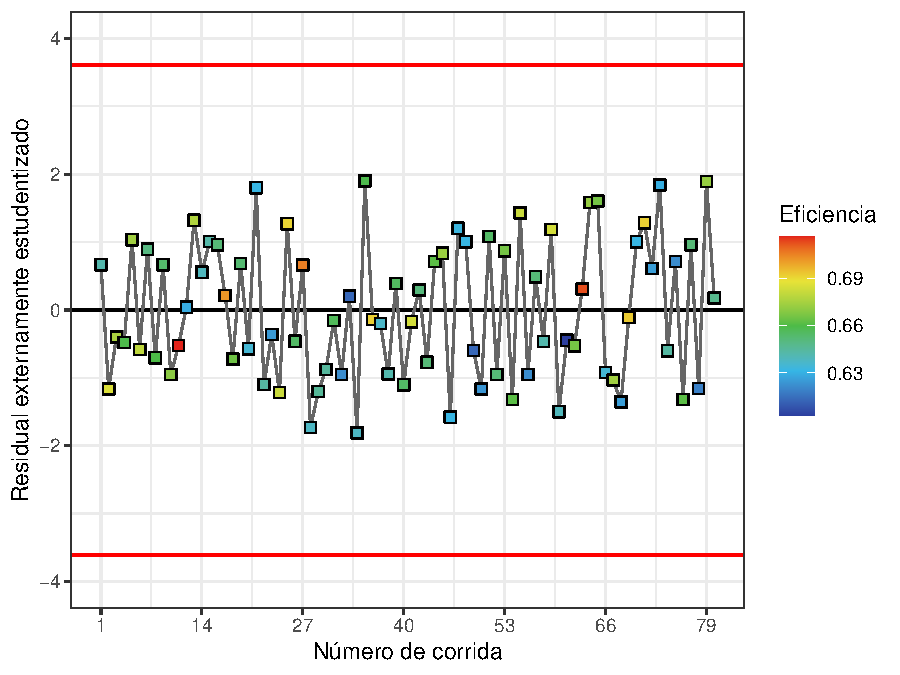
\includegraphics[width=\textwidth]{Articulo_Revista/Figs/fig9d_rext_corrida.pdf}\\
  {\small (d)}
\end{minipage}
\caption{Gráficos de diagnóstico: (a) probabilidad normal de los residuales externamente estudentizados, (b) eficiencia predicha frente a observada, (c) residuales internamente estudentizados y (d) residuales externamente estudentizados frente al número de corrida. Código: sección~10 de \texttt{mod\_lin.R}.}
\label{fig:diagnosticos}
\end{figure}

\begin{itemize}
  \item \textbf{(a) Probabilidad normal.} Cada residual se ubica frente al percentil que le correspondería si los residuales vinieran de una distribución normal; si la normalidad se cumple, los puntos quedan cerca de la recta. En la parte central los puntos siguen la recta. En los extremos se separan un poco y forman una S suave: los residuales más grandes en valor absoluto son menos extremos de lo que se esperaría con una normal, es decir, las colas son algo más livianas. La desviación es leve y no hay puntos aislados, así que el supuesto de normalidad es razonable.
  \item \textbf{(b) Predicha frente a observada.} Cada punto compara la eficiencia que predice el modelo con la que se midió. Si el modelo predice bien, los puntos quedan sobre la diagonal $y = x$. Aquí están muy cerca de ella en todo el rango, de 0.60 a 0.72, sin curvas ni zonas donde el modelo se equivoque de forma sistemática.
  \item \textbf{(c) Residuales internamente estudentizados frente al número de corrida.} Los puntos saltan de arriba abajo alrededor de cero, sin tendencia y sin que la dispersión crezca o se reduzca a lo largo de las corridas. Esto es compatible con errores independientes y de varianza constante. Todos están entre $-2$ y $2$, lejos de los límites de $\pm 3$ (líneas rojas) que usa Design Expert para señalar valores sospechosos.
  \item \textbf{(d) Residuales externamente estudentizados frente al número de corrida.} Las líneas rojas están en $\pm 3.61$. Ese límite es más amplio que $\pm 3$ porque tiene en cuenta que se revisan 80 corridas a la vez: con tantas corridas, alguna podría superar $\pm 3$ solo por azar (es el valor crítico $t$ con 60 grados de libertad y corrección de Bonferroni). Ninguna corrida lo supera, así que no hay observaciones atípicas.
\end{itemize}

En conjunto, los diagnósticos no muestran problemas con los supuestos del modelo.

\subsection{Superficies de respuesta}

Con el modelo ajustado se puede predecir la eficiencia en cualquier combinación de valores dentro de la región del experimento. La Figura~\ref{fig:contornos} muestra esas predicciones como gráficos de contorno, en función del ángulo y del diámetro, con la distancia fija en 50~mm y un panel para cada combinación de rodete y número de boquillas (sección~11 de \texttt{mod\_lin.R}). Se leen como un mapa topográfico: cada franja de color agrupa las combinaciones con la misma eficiencia predicha, las líneas negras separan franjas que difieren en 0.01 y los puntos rojos son las corridas del diseño con distancia de 50~mm. La Figura~\ref{fig:superficies} presenta las mismas predicciones como superficies en tres dimensiones, que reproducen la Figura~10 del artículo original.

\begin{figure}[ht]
\centering
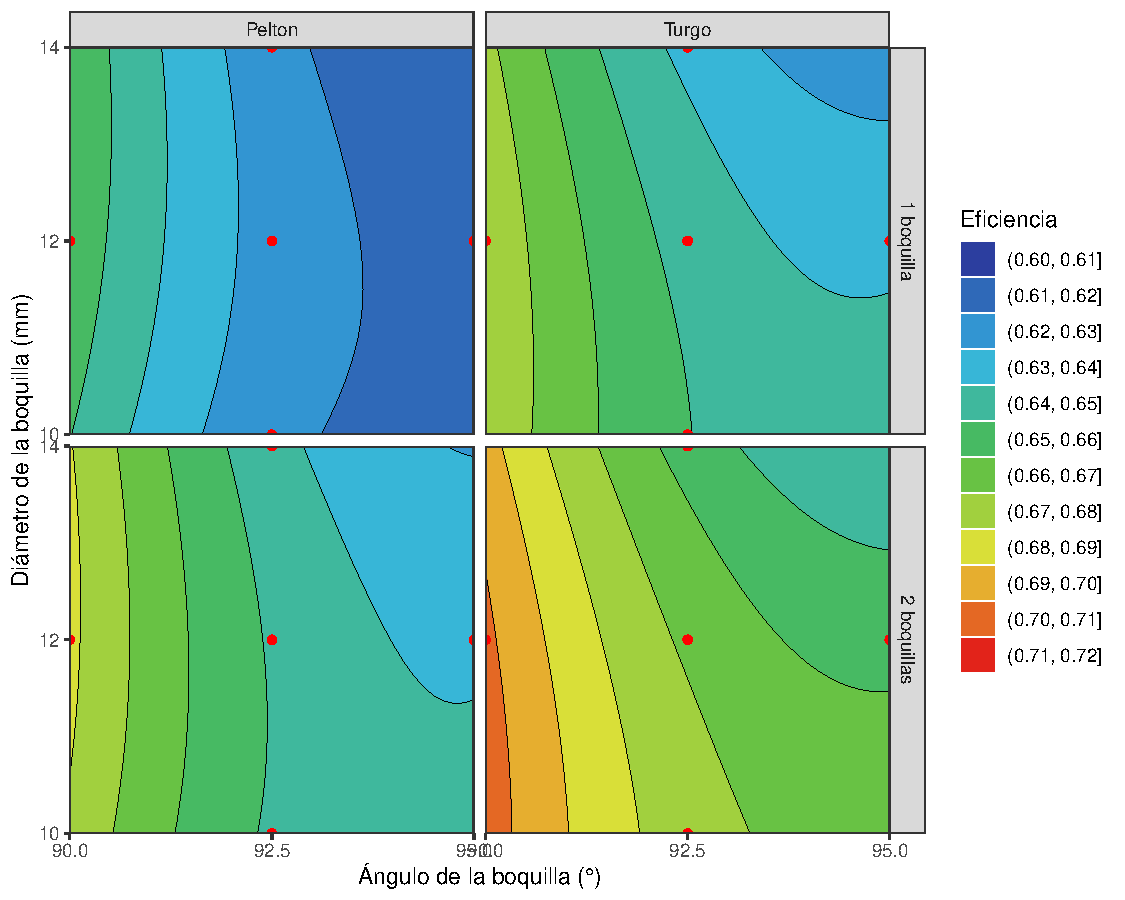
\includegraphics[width=0.8\textwidth]{Articulo_Revista/Figs/fig10_contornos.pdf}
\caption{Contornos de la eficiencia predicha según el ángulo y el diámetro de la boquilla, con la distancia en 50~mm, para cada tipo de rodete (columnas) y número de boquillas (filas). Código: sección~11 de \texttt{mod\_lin.R}.}
\label{fig:contornos}
\end{figure}

\begin{figure}[ht]
\centering
\begin{minipage}[b]{0.42\textwidth}
  \centering
  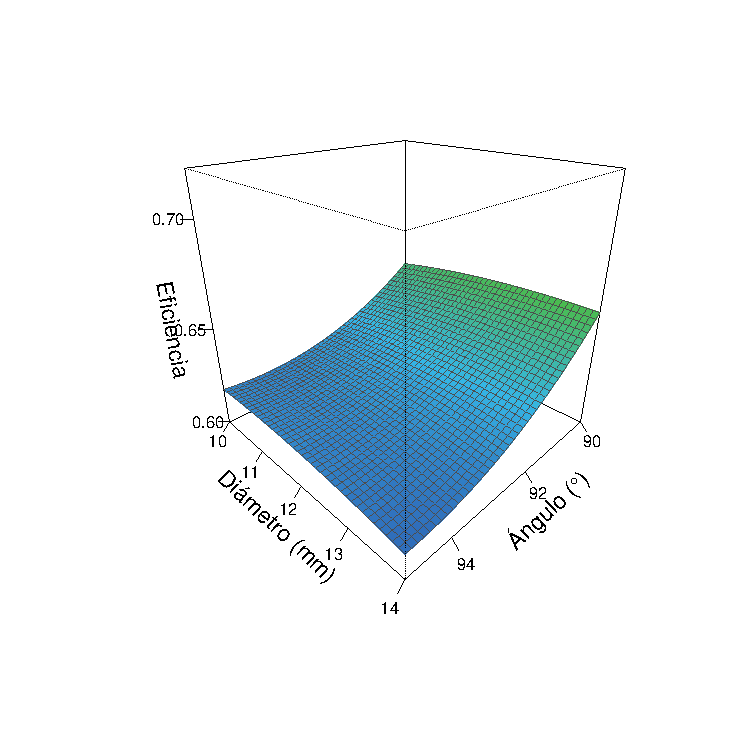
\includegraphics[width=\textwidth]{Articulo_Revista/Figs/fig10a_superficie_pelton_1.pdf}\\
  {\small (a) Pelton, 1 boquilla}
\end{minipage}\hspace{0.04\textwidth}
\begin{minipage}[b]{0.42\textwidth}
  \centering
  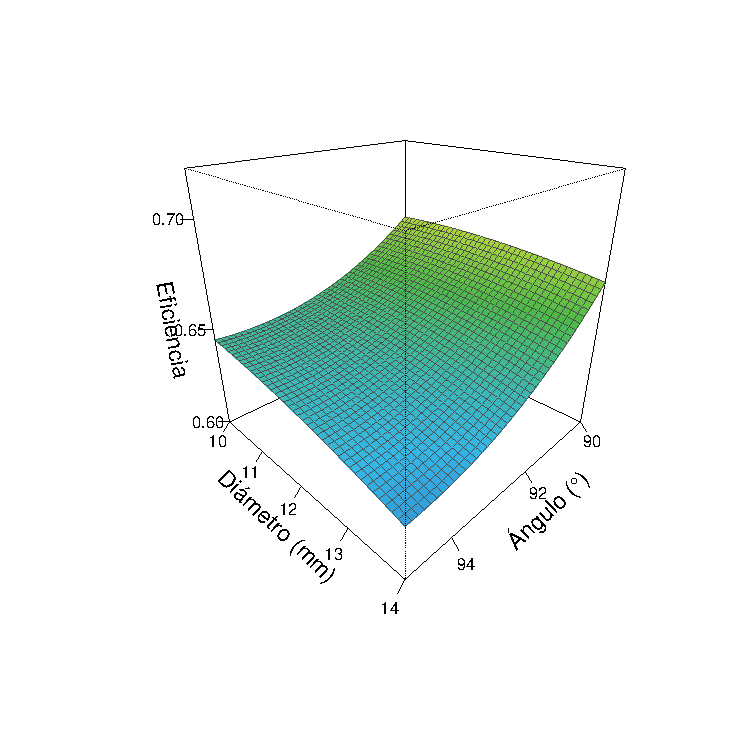
\includegraphics[width=\textwidth]{Articulo_Revista/Figs/fig10b_superficie_turgo_1.pdf}\\
  {\small (b) Turgo, 1 boquilla}
\end{minipage}\\[6pt]
\begin{minipage}[b]{0.42\textwidth}
  \centering
  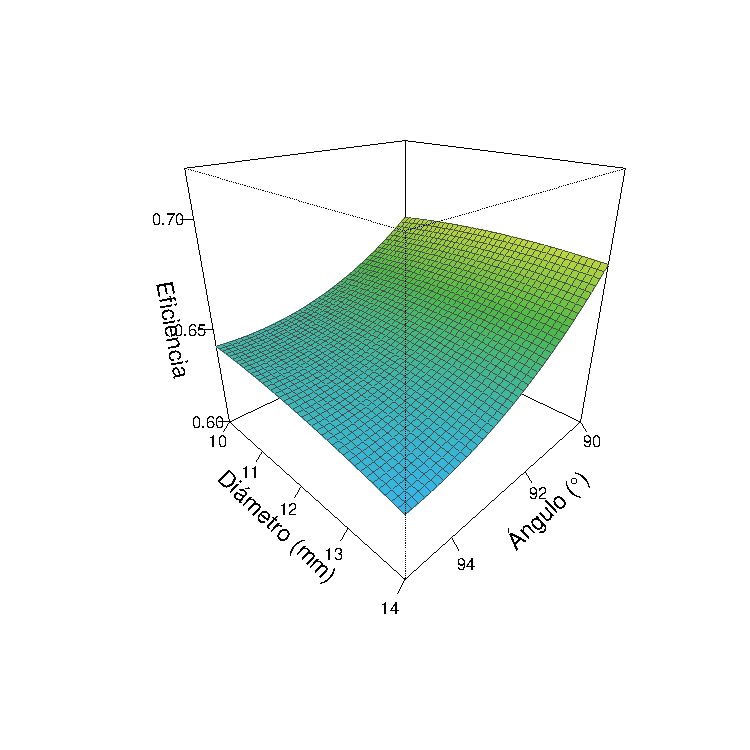
\includegraphics[width=\textwidth]{Articulo_Revista/Figs/fig10c_superficie_pelton_2.pdf}\\
  {\small (c) Pelton, 2 boquillas}
\end{minipage}\hspace{0.04\textwidth}
\begin{minipage}[b]{0.42\textwidth}
  \centering
  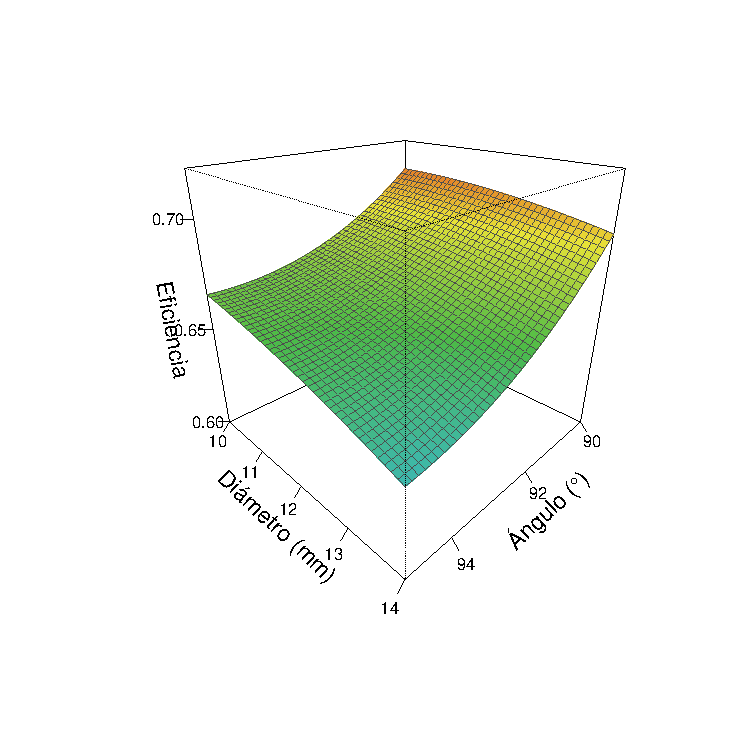
\includegraphics[width=\textwidth]{Articulo_Revista/Figs/fig10d_superficie_turgo_2.pdf}\\
  {\small (d) Turgo, 2 boquillas}
\end{minipage}
\caption{Superficies de respuesta de la eficiencia predicha según el ángulo y el diámetro de la boquilla, con la distancia en 50~mm. Código: sección~11 de \texttt{mod\_lin.R}.}
\label{fig:superficies}
\end{figure}

En los cuatro paneles la eficiencia predicha aumenta hacia la izquierda, es decir, hacia 90°, y las franjas son más angostas cerca de 90° que cerca de 95°: la eficiencia cambia rápido al alejarse de 90° y luego se estabiliza, que es el efecto del término cuadrático del ángulo. En el Pelton las franjas son casi verticales, lo que indica que el diámetro casi no cambia la eficiencia. En el Turgo las franjas se inclinan y la eficiencia es mayor con diámetros pequeños, sobre todo cerca de 95°, como lo indicaban las interacciones $BD$ y $AB$. Los paneles de abajo (dos boquillas) y los de la derecha (Turgo) alcanzan colores más altos, y la eficiencia predicha más alta de la figura está en el Turgo con dos boquillas, con 90° y diámetros pequeños.

\subsection{Condición de máxima eficiencia}

\citet{Lakdawala2025} reportan como condición óptima el rodete Turgo con dos boquillas, 95°, 14~mm y 40~mm, con una eficiencia predicha de 0.6619. El modelo replicado da la misma predicción en ese punto, y la corrida 53, hecha en esas condiciones, tuvo una eficiencia de 0.6655 (sección~12 de \texttt{mod\_lin.R}).

Sin embargo, ese no es el máximo del modelo. Al evaluar el modelo en una rejilla fina dentro de la región del experimento, la eficiencia predicha máxima de cada combinación de rodete y número de boquillas se alcanza siempre con 90° y 40~mm (Tabla~\ref{tab:maximos}). El máximo global es 0.7190, en el Turgo con dos boquillas, con 90°, 10.6~mm y 40~mm. Esto coincide con el análisis descriptivo, donde la eficiencia media más alta se dio con 90°, y con la corrida 11 (90°, 10~mm, 40~mm, Turgo con dos boquillas), que tuvo la mayor eficiencia observada, 0.7165. El artículo no detalla los criterios de su optimización, así que no es posible saber por qué su punto óptimo está en 95°.

\begin{table}[ht]
\centering
\caption{Condición de máxima eficiencia predicha dentro de la región del experimento para cada combinación de rodete y número de boquillas.}
\label{tab:maximos}
\begin{tabular}{llcccc}
\toprule
Rodete & Boquillas & Ángulo (°) & Diámetro (mm) & Distancia (mm) & Eficiencia predicha \\
\midrule
Pelton & 1 & 90 & 14.0 & 40 & 0.6711 \\
Pelton & 2 & 90 & 13.2 & 40 & 0.6935 \\
Turgo  & 1 & 90 & 11.6 & 40 & 0.6941 \\
Turgo  & 2 & 90 & 10.6 & 40 & 0.7190 \\
\bottomrule
\end{tabular}
\end{table}


\clearpage % para que todas las figuras queden antes de las referencias
% ------------------------------------------------------------
% Disponibilidad de datos y código
% ------------------------------------------------------------

\subsection*{Disponibilidad de datos y código}

Los datos y el código en R usados en este trabajo están disponibles en el repositorio \url{https://github.com/mariasaurius/Articulo_regresion}: \texttt{anal\_descrip.R} contiene el análisis descriptivo y \texttt{mod\_lin.R} la réplica del modelo de regresión.


%-------------------------------------------------------------------------------

%-------------------------------------------------------------------------------
\bibliography{mis_referencias}

%-------------------------------------------------------------------------------
\appendix
\section{Glosario}
\label{sec:glosario}
% ------------------------------------------------------------
% Apéndice A. Glosario
% ------------------------------------------------------------

% ---------------------------------------------------
% Glosario de términos usados en Lakdawala et al. (2025)
% Formato: \item[Término] (\textit{término en inglés}) definición
% ---------------------------------------------------

Este glosario reúne los términos técnicos que aparecen en \citet{Lakdawala2025}. Entre paréntesis se indica el término en inglés usado en el artículo y, cuando aplica, su notación.

\subsection*{Turbinas y banco de pruebas}

\begin{description}

\item[Pico central hidroeléctrica] (\textit{pico hydro}) Instalación hidroeléctrica de muy pequeña potencia, pensada para abastecer cargas aisladas, fuera de la red eléctrica (\textit{off-grid}). El prefijo \textit{pico} se refiere al rango de potencia del generador.

\item[Turbina de impulso] (\textit{impulse turbine}) Turbina en la que el agua sale de una boquilla convertida en un chorro de alta velocidad y transmite su energía cinética al rodete al golpear los cangilones, a presión atmosférica. Las turbinas Pelton y Turgo son de este tipo.

\item[Turbina Pelton] (\textit{Pelton Turbine Runner}, PTR) Turbina de impulso cuyos cangilones tienen dos cavidades separadas por una arista central que divide el chorro en dos mitades, que salen por los costados del cangilón.

\item[Turbina Turgo] (\textit{Turgo Turbine Runner}, TTR) Turbina de impulso con cangilones de una sola cavidad, más angostos que los Pelton, en la que el chorro entra por una cara del rodete y sale por la cara opuesta.

\item[Rodete] (\textit{runner}) Rueda giratoria de la turbina formada por el disco y los cangilones; convierte la energía del chorro en giro del eje.

\item[Cangilón] (\textit{bucket}) Cada una de las cucharas o álabes del rodete donde golpea el chorro. En el estudio se fabricaron por impresión 3D.

\item[Arista divisoria] (\textit{splitter}) Borde central del cangilón que parte el chorro. Su ángulo ($\theta_s$) fue de 30° en el rodete Pelton y de 15° en el Turgo.

\item[Diámetro primitivo] (\textit{pitch circle diameter}, PCD) Diámetro de la circunferencia del rodete sobre la que el chorro golpea los cangilones. Fue de 100~mm en los dos rodetes.

\item[Distancia boquilla-rodete] (\textit{nozzle standoff distance}, $N_{sod}$ o SOD) Distancia entre la punta de la boquilla y el punto donde el chorro golpea el cangilón. Se probaron 40, 50 y 60~mm.

\item[Caída o cabeza] (\textit{head}, $H$) Altura de agua disponible, que determina la energía por unidad de peso del agua. En el estudio se mantuvo constante en 10~m.

\item[Caudal] (\textit{flow rate}, $Q$) Volumen de agua que pasa por la turbina por unidad de tiempo; se midió con un caudalímetro electromagnético.

\item[Velocidad angular] (\textit{angular velocity}, $\omega$) Velocidad de giro del rodete; se midió con un tacómetro sin contacto.

\item[Eficiencia hidráulica] (\textit{hydraulic efficiency}, $\eta_h$) Fracción de la potencia hidráulica del agua que el rodete convierte en potencia en el eje:
\[
\eta_h = \frac{T\,\omega}{\rho\, g\, Q\, H},
\]
donde $\rho$ es la densidad del agua y $g$ la aceleración de la gravedad. Es la variable respuesta de este trabajo.

\item[PLA] (\textit{Polylactic Acid}) Ácido poliláctico, plástico biodegradable usado para imprimir en 3D los cangilones.

\end{description}


\end{document}
